\documentclass[letterpaper, twoside]{article}
\usepackage{mystyle}

\newtcolorbox{myboxWithTitle}[1]{colback=red!5!white,
	colframe=red!75!black,fonttitle=\bfseries,
	title={#1}}

\newtcolorbox{mybox}{colback=red!5!white,
	colframe=red!75!black}

\newenvironment{leading}[1]{\begin{spacing}{#1}}{\end{spacing}}		%interlinia  
\newcommand{\version}{v0.2.0}

\begin{document}

%opening
\author{
	Jakub Głuszek\\
}
\title{Zaawansowane techniki obiektowe\\Laboratorium}
\date{\today}


\makeatletter
\newcommand{\linia}{\rule{\linewidth}{0.4mm}}
\renewcommand{\maketitle}{\begin{titlepage}
		\vspace*{1cm}
		\begin{center}\large
			Wyższa Szkoła Bankowa\\
			Wydział Finansów i Zarządzania\\
			Informatyka Inżynierska\\
			Studia II stopnia, semestr 2/3\\
			Gdańsk
		\end{center}
		\vspace{3cm}
		\noindent
		\begin{center}
			\Huge \textbf{\textsc{\@title}}
		\end{center}
		\vspace{0.5cm}
		\begin{center}
			\Large \version
		\end{center}		
		\vspace{1cm}
		\begin{flushright}
			\begin{minipage}{5cm}
				\textit{\small Autor:}\\
				\normalsize \textsc{\@author} \par
			\end{minipage}
			\vspace{1cm}
		\end{flushright}
		
		\begin{center}
			
\includegraphics[width=.4\linewidth]{images/logo}
		\end{center}
		
		\vspace*{\stretch{6}}
		\begin{center}
			\Large\@date
		\end{center}
	\end{titlepage}%
}

\begin{titlepage}
	\maketitle
\end{titlepage}
\tableofcontents
\newpage


% Intro - luźne przemyślenia
%- Chcemy aby każdy członek zespołu stosował podobne zasady, wzorce i nazewnictwo. 
%- Wzorce i struktura są często dużo ważniejsze niż same algorytmy. 
%- Zazwyczaj temat wzorców projektowych, zasad SOLID, TDD czy refaktoringu pojawia się podczas rozmów kwalifikacyjnych. 
%- Wzorce i wspominane zasady SOLILD pozwalają odpowiedziec na pytanie jak podzielić projekt na niezależne komponenty, tak aby można było łatwo je rozszerzać i zamieniać, bez konieczności wprowadzania zmian w pozostałych komponentach. Dobry podział pozwala na szybsze znajdowanie błędów w oprogramowaniu. Jeżeli przepływ informacji jest prosty nie powinno być ciężko dowiedzieć się czy błąd znajduje się w warstwie logiki biznesowej, w kontrolerze czy widoku.
%- Z wzorcem Singleton może istnieć problem, że mamy dwa takie obiekty, które ze sobą rozmawiają. Przepływ informacji jest dwukierunkowy, który sprawia, że ciężej jest zrozumieć program i go debugować. Zazwyczaj zależy nam na jednokierunkowym przepływie informacji.
%- Obiekty modelu powinny zawierać jedynie takie zachowania, które bezpośrednio zmieniają ich stan. Nie powinny one zawierać logiki biznesowej.

\section{Zasady SOLID}

W publikacji \texttt{Design Principles and Design Patterns} Robert C. Martin opisał 5 zasad SOLID, które pomagają uzyskać lepszy, bardziej zrozumiały i łatwiejszy w utrzymaniu oraz rozbudowie kod. Są one również trzonem metodologi takich jak Agile czy programowanie adaptywne. W kolejnych podrozdziałach zostaną one po kolei opisane. 

\subsection{SRP - Zasada pojedynczej odpowiedzialności (ang. \textbf{S}OLID)}\label{lab1/sec/srpPrinciple}

Pierwsza z pięciu zasad mówi, że każdy moduł, zestaw, klasa czy metoda powinna posiadać pojedynczy obszar odpowiedzialności (przyczynę zmian).  W momencie zmian wymagań, określa się jakie klasy są odpowiedzialne za dane wymagania i to te kasy się modyfikuje. Jeśli istnieją co najmniej dwa niezależne powody mogące wymusić zmianę w danej klasie, to dana klasa rozciąga się na więcej niż jeden obszar odpowiedzialności. W~przypadku naruszenia zasady SRP zmiany w dwóch różnych wymaganiach implikują modyfikację w jednej, tej samej klasie. 
%Niepożądane są tzw. ,,boskie klasy'' (ang. God classes), które są odpowiedzialne za wiele rzeczy. 

\begin{myboxWithTitle}{Zasada pojedynczej odpowiedzialności}
	Żadna klasa nie może być modyfikowana z więcej niż jednego powodu.
\end{myboxWithTitle}

Wyobraźmy sobie sytuację, w której klasa rysująca na ekranie figurę geometryczną np. \texttt{Rectangle} jest odpowiedzialna zarówno za wspomniane rysowanie, ale również za wyznaczanie pola powierzchni danej figury. Jakie konsekwencje to za sobą niesie? Jeśli dwa zestawy np. interfejsu użytkownika \texttt{UI} oraz jakiś inny korzystający jedynie z operacji liczenia pola powierzchni będą związane z klasą \texttt{Rectangle} to zmiana wynikająca z wymagań związanych z \texttt{UI} może pociągać ryzyko nieprawidłowego działania w drugim zestawie. Aby nie naruszyć zasady SRP należałoby stworzyć dwie osobne klasy: jedną rysująca figurę i drugą liczącą pole powierzchni. Pierwsza z~nich mogłaby wykorzystywać tę pierwszą. 

Oczywiście należy zawsze mieć na uwadze, że rozdrabniać klasy na coraz mniejsze typy można prawie w~nieskończoność. Może to prowadzić do nadmiernego skomplikowania projektu. Konieczne jest branie pod uwagę wymagań i ich potencjalnych zmian.

Jako przykład przeanalizujmy interfejs \texttt{IModem}.
\begin{lstlisting}[caption={Naruszenie zasady SRP}, label={lab1/lst/srpViolationModem}]
public interface IModem
{
	void Dial(string phoneNumber);
	void Hangup();
	void Send(char c);
	char Recieve();
}
\end{lstlisting}
Widać, że interfejs mógłby zostać podzielony na dwa obszary odpowiedzialności. Jeden odpowiadający za nawiązywanie i zrywanie połączeń, drugi natomiast za same funkcje komunikacyjne. Klasy klienckie mogłyby wykorzystywać klasę implementującą dwa interfejsy np. \texttt{IDataChannel} i \texttt{IConnection} i tym samym uzależnić się tylko od jednego z obszarów odpowiedzialności. 
%Tutaj konieczne jest przeanalizowanie wymagań, ponieważ podział interfejsu na dwa zawierające odpowiednio \texttt{Dial} i \texttt{Hangup} oraz \texttt{Send} i \texttt{Recieve} może nie być potrzebny, jeśli zmiany w aplikacji nie wpływają na zmiany w~metodach zarządzających wykonywaniem połączeń.
% [DataChannel]^-.-[ModemImplementation]
% [Connection]^-.-[ModemImplementation]
%[<<interface>>;DataChannel|+send(c:char);+recv():char]
%[<<interface>>;Connection|+dial(pno: String);+hangup()]

%\subsubsection{Zadanie 1}
%\begin{lstlisting}[caption={Naruszenie zasady SRP}, label={lab1/lst/srpViolationEmployee}]
%class Employee()
%{
%	public void CalculatePay();
%	public void ReportHours();
%	public void Store();
%}
%\end{lstlisting}
%W powyższym przykładzie została naruszona zasada SRP, zaproponuj sposób rozdzielenia odpowiedzialności tej klasy. 
%
%Utwórz nowy projekt .NET 5.0 i dodaj do niego klasy, które pozwolą na implementację zachowań klasy \texttt{Employee} tak, aby zachować zasadę SRP.

% Zakładamy, że te trzy metody są wykorzystywane przez innego aktora. Np. CalculatePay przez dział księgowości, ReportHours przez dział kadr, a Store() przez dział administrowania bazami danych. Umieszczając to w jednej klasie zostały połączone odpowiedzialności trzech aktórów. 
% Dodatkowo złączenia (merge) w gitcie są dość ryzykowne, a dzieje się tak często jeśli dwóch programistów pracuje nad tą samą klasą.


% Podejść do problemu można na trzy sposoby:
% 1. Trzy osobne klasy, PayCalculator, HourReporter oraz EmployeeSaver, które współdzielą dostęp do klasy EmployeeData (struktura danych)
% 2. Rozwinięcie punktu nr 1. Zastosować wzorzec Fasada, która tworzy i deleguje zadania wywołania do odpowiednich klas i ich funkcji. Pozwala to uniknąć problemu, konieczności tworzenia i żąglowania trzema obiektami. 
% 3. Utrzymać reguły biznesowe blisko właściwych danych. Klasa Employee może stać fasadą dla pomniejszych funkcji. Może zawierać klasy (lepiej referencje do interfejsów) do HourReporter i EmployeeSaver. Sama natomiast może posiadać employeeData, CalculatePay(), ReportHours(), Store() - te dwie ostatnie mogłyby delegować zadania do odpowiednich implementacji przekazanych np. jako argumenty konstruktora. 

% Reguły biznesowe jak i mechanizmy wiedzialności nigdy nie powinny być ze sobą łączone. Powodu do ich zmian są różne. 
% Możemy powyższą klasę podzielić na trzy mniejsze klasy:
%\begin{itemize}
%	\item PayCalculator z metodą CalculatePay,
%	\item HourReporter z metodą ReportHours,
%	\item EmployeeRepository z metodą SaveEmployee.
%\end{itemize}
%Każda z tych klas może korzystać z encji \texttt{EmployeeData}.



\subsubsection{Zadanie 1}

Poniżej przedstawiony fragment kodu\cite{adaptatywny_kod_hall} zawiera klasę\ref{lab1/lst/srpViolationEmployee} z metodą \texttt{ProcessTrades}, która wyraźnie narusza zasadę SRP. Utwórz nowy projekt .NET 5.0 i dodaj do niego poniższą klasę w~osobnym pliku. Nazwij ten plik \texttt{TradeProcessor.cs}.

\begin{lstlisting}[caption={Naruszenie zasady SRP}, label={lab1/lst/srpViolationEmployee}]
public class TradeProcessor
{
	public void ProcessTrades(Stream stream)
	{
		// read rows
		var lines = new List<string>();
		using (var reader = new StreamReader(stream))
		{
			string line;
			while ((line = reader.ReadLine()) != null) { }
			lines.Add(line);
		}
		
		var trades = new List<TradeRecord>();
		var lineCount = 1;
		foreach (var line in lines)
		{
			var fields = line.Split(new char[] { ',' });
			if (fields.Length != 3)
			{
				Console.WriteLine("WARN: Line {0} malformed. Only {1} field(s) found.",
				lineCount, fields.Length);
				continue;
			}
			if (fields[0].Length != 6)
			{
				Console.WriteLine("WARN: Trade currencies on line {0} malformed: '{1}'", lineCount, fields[0]);
				continue;
			}
			if (!int.TryParse(fields[1], out int tradeAmount))
			{
				Console.WriteLine("WARN: Trade amount on line {0} not a valid integer: '{1}'", lineCount, fields[1]);
			}
			if (!decimal.TryParse(fields[2], out decimal tradePrice))
			{
				Console.WriteLine("WARN: Trade price on line {0} not a valid decimal: '{1}'", lineCount, fields[2]);
			}
			var sourceCurrencyCode = fields[0].Substring(0, 3);
			var destinationCurrencyCode = fields[0].Substring(3, 3);
			// calculate values
			var trade = new TradeRecord
			{
				SourceCurrency = sourceCurrencyCode,
				DestinationCurrency = destinationCurrencyCode,
				Lots = tradeAmount / LotSize,
				Price = tradePrice
			};
			trades.Add(trade);
			lineCount++;
		}
		using (var connection = new System.Data.SqlClient.SqlConnection("Data Source = (local); Initial Catalog = TradeDatabase; Integrated Security = True"))
		{
			connection.Open();
			using (var transaction = connection.BeginTransaction())
			{
				foreach (var trade in trades)
				{
					var command = connection.CreateCommand();
					command.Transaction = transaction;
					command.CommandType = System.Data.CommandType.StoredProcedure;
					command.CommandText = "dbo.insert_trade";
					command.Parameters.AddWithValue("@sourceCurrency", trade.
					SourceCurrency);
					command.Parameters.AddWithValue("@destinationCurrency", trade.
					DestinationCurrency);
					command.Parameters.AddWithValue("@lots", trade.Lots);
					command.Parameters.AddWithValue("@price", trade.Price);
					command.ExecuteNonQuery();
				}
				transaction.Commit();
			}
			connection.Close();
		}
		Console.WriteLine("INFO: {0} trades processed", trades.Count);
	}
	private readonly float LotSize = 100000f;
}
\end{lstlisting}
Dodatkowo utwórz klasę typu \texttt{TradeRecord}:
\begin{lstlisting}[caption={Klasa \texttt{TradeRecord}}]
public class TradeRecord
{
	public string SourceCurrency { get; set; }
	public string DestinationCurrency { get; set; }
	public float Lots { get; set; }
	public decimal Price { get; set; }
}
\end{lstlisting}


W powyżej klasie można na pierwszy rzut oka wydzielić trzy odpowiedzialności:
\begin{enumerate}
	\item odczytywanie dane,
	\item konwertowanie danych na obiekty typu \texttt{TradeRecord},
	\item utrwalanie danych.
\end{enumerate}

Dodaj do projektu trzy interfejsy w trzech osobnych plikach:
\begin{lstlisting}
public interface ITradeDataProvider
{
	IEnumerable<string> GetTradeData();
}
\end{lstlisting}
\begin{lstlisting}
public interface ITradeParser
{
	IEnumerable<TradeRecord> Parse(IEnumerable<string> lines);
}
\end{lstlisting}
\begin{lstlisting}
public interface ITradeStorage
{
	void Persist(IEnumerable<TradeRecord> trades);
}
\end{lstlisting}
Każdy z powyższych interfejsów będzie odpowiadał jednej z trzech odpowiedzialności klasy \texttt{TradeProcessor}. Docelowo każda zostanie umieszczona w~osobnej klasie.

Następnie utwórz trzy klasy implementujące odpowiednio trzy powyższe interfejsy:
\begin{lstlisting}
public class StreamTradeDataProvider : ITradeDataProvider
{
	private readonly Stream stream;
	public StreamTradeDataProvider(Stream stream) => this.stream = stream;
	
	public IEnumerable<string> GetTradeData()
	{
		//...
	}
}
\end{lstlisting}
\begin{lstlisting}
public class SimpleTradeParser : ITradeParser
{	
	public IEnumerable<TradeRecord> Parse(IEnumerable<string> lines)
	{
		//...
	}
}
\end{lstlisting}
\begin{lstlisting}
public class DbTradeStorage : ITradeStorage
{	
	public void Persist(IEnumerable<TradeRecord> trades)
	{
		//..
	}
}
\end{lstlisting}

Przenieś fragmenty kodu z metody \texttt{ProcessTrades} klasy \texttt{TradeProcessor} do powyższych metod. Do klasy \texttt{TradeProcessor} dodaj konstruktor, przyjmujący trzy obiekty implementujące powyższe interfejsy. Dodaj do \texttt{TradeProcessor} trzy prywatne pola i przypisz do nich przekazane przez konstruktor argumenty. W~metodzie \texttt{ProcessTrades} wykorzystaj obiekty przechowywane w~tych polach w~celu przetworzenia sprzedaży. 
\begin{lstlisting}
public class TradeProcessor
{
	public TradeProcessor(ITradeDataProvider tradeDataProvider,
	ITradeParser tradeParser,
	ITradeStorage tradeStorage)
	{
		this.tradeDataProvider = tradeDataProvider;
		this.tradeParser = tradeParser;
		this.tradeStorage = tradeStorage;
	}

	public void ProcessTrades()
	{
		// read rows
		var lines = tradeDataProvider.GetTradeData();
		var trades = tradeParser.Parse(lines);
		tradeStorage.Persist(trades);
	}
	
	private readonly ITradeDataProvider tradeDataProvider;
	private readonly ITradeParser tradeParser;
	private readonly ITradeStorage tradeStorage;
}
\end{lstlisting}

Z metody \texttt{Parse} znajdującej się w klasie \texttt{SimpleTradeParser} można wydzielić dodatkowe dwie odpowiedzialności: walidacji oraz mapowania pól na obiekt typu \texttt{TradeRecord}. Dodaj do projektu dodatkowe dwa interfejsy:
\begin{lstlisting}
public interface ITradeValidator
{
	bool Validate(string[] fields, int lineCount);
}
\end{lstlisting}
oraz 
\begin{lstlisting}
public interface ITradeMapper
{
	TradeRecord Map(string[] fields);
}	
\end{lstlisting}

Dalej utwórz dwie nowe klasy implementujące te interfejsy:
\begin{lstlisting}
public class SimpleTradeValidator : ITradeValidator
{	
	public bool Validate(string[] fields, int lineCount)
	{
		//...
	}
}
\end{lstlisting}
\begin{lstlisting}
public class SimpleMapper : ITradeMapper
{
	public TradeRecord Map(string[] fields)
	{
		//...
	}
}	
\end{lstlisting}

Analogicznie jak wcześniej przenieś fragmenty kodu z metody \texttt{Parse} klasy \texttt{SimpleTradeParser} do odpowiednich klas. W~klasie \texttt{SimpleTradeParser} dodaj konstruktor przyjmujący obiekty implementujące powyższe interfejsy. Przypisz te argumenty do prywatnych pól klasy. Na koniec wykorzystaj te obiekty w~metodzie \texttt{Parse}.
\begin{lstlisting}
public class SimpleTradeParser : ITradeParser
{
	private readonly ITradeValidator tradeValidator;
	private readonly ITradeMapper tradeMapper;
	
	public SimpleTradeParser(ITradeValidator tradeValidator, ITradeMapper tradeMapper)
	{
		this.tradeValidator = tradeValidator;
		this.tradeMapper = tradeMapper;
	}

	//...
}	
\end{lstlisting}

Na koniec można się pokusić o dodanie interfejsu \texttt{ILogger}, tak aby uniezależnić klasy od sposobu logowania informacji o~błędach.
\begin{lstlisting}
public interface ILogger
{
	void LogWarning(string message, params object[] args);
	void LogInfo(string message, params object[] args);
	void LogError(string message, params object[] args);
}	
\end{lstlisting}
I klasy go implementującej:
\begin{lstlisting}
public class CustomLogger : ILogger
{
	public void LogError(string message, params object[] args) => Console.WriteLine("ERROR: " + message, args);
	public void LogInfo(string message, params object[] args) => Console.WriteLine("INFO: " + message, args);
	public void LogWarning(string message, params object[] args) => Console.WriteLine("WARN: " + message, args);
}	
\end{lstlisting}
Teraz można dodać parametr w konstruktorze klas: \texttt{SimpleTradeValidator} i \texttt{DbTradeStorage} typu \texttt{ILogger} i przypisać go prywatnych pól tych klas. Dalej należy zamienić wywołania metody \texttt{Console.WriteLine}, odpowiednimi metodami obiektu implementującego \texttt{ILogger.}

Dzięki powyższym krokom będzie istniała możliwość zmiany rejestracji komunikatów w przypadku zmiany wymagań. Wystarczy dodać nową klasę implementującą interfejs \texttt{ILogger}, albo wykorzystać wzorzec Adapter\ref{sec/lab3/adapter} do dostosowania innych, już istniejących implementacji


Przeprowadzone zmiany nie zmieniły funkcjonalności kodu. %Sprawdzić to można np. korzystając ze złotego wzorca.
Jednak można teraz go zdecydowanie łatwiej rozszerzać, dostosowywać do nowych wymagań. Łatwo można zmienić źródło danych wejściowych np. na z usługi WWW, wystarczy napisać nową klasę implementującą \texttt{ITradeDataProvider}. Analogicznie łatwo będzie można zmienić format danych wejściowych, reguły walidacji, sposób logowania informacji, ostrzeżeń czy błędów.

% Inny przykład z Adaptive Code:
% klasa czytała dane ze strumienia, prasowała i walidowała każde pole i przechowywała w liście typu \texttt{TradeRecord}, dodatkowo wykonywała logowania do konsoli a następnie zapisywała te dane do bazy danych. 
% Jeśli nagle stwierdzimy, że nie chcemy korzystać ze strumienia a z WebAPI konieczna będzie zmiana tej klasy. Analogicznie jeśli zmieni się format danych, zasady walidacji, logowania czy będziemy korzystać z innej bazy danych. Zasada SRP została tutaj naruszona wielokrotnie. 
% Refaktoryzacja mogłaby polegać na utworzeniu trzech interfejsów: \texttt{ITradeDataProvider, ITradeParser oraz ITradeStorage} i korzystanie z nich przez klasę \texttt{TradeProcessor}. Klasy implemntujące te interfejsy będą odpowiedzialne za różne obszary odpowiedzialności. Obiekty można wstrzyknąć przez konstrutkor i dalej już klasa \texttt{TradeProcessor} może z nich korzystać przetwarzająć operacje (będzie pełniła role swego rodzaju fasady). Implementacje mogą znajdować się w tym samym zestawie, jednak jeśli korzystalibyśmy z zewnętrznych zależności (firm trzecich) należy wtedy je umieścić z osobnym zestawie. Np. jeśli chcemy korzystać z Dapper'a zamiast ADO.NET należy stworzyć zestawe Services.Dapper, który będzie implementował ITradeStorage nazwany DapperTradeStorage. Ważne, aby zależności nie były zaszyte w interfejsie, a jedynie wstrzykiwane przez konstruktor. Interfejs powinnien być czysty. Można dodać dodatkowe abstrakcje  np. \texttt{ParseTrades} wykonuje zarówno walidację jak i mapowanie. Tak więc podział można ponownie przeprowadzić i wyodrębnić dwa dodatkowe interfejsy \texttt{ITradeMapper} oraz \texttt{ITradeValidator}. Może tak postępować tak długo, aż każda klasa będzie posiadała tylko jedną odpowiedzielność. Jeśli omawiana klasa dodatkowo przeprowadzała logowanie to dobrze będzie stworzyć adapter na jedną z popularnych klas do logowania np. NLog.

\subsection{OCP - Zasada otwarte - zamknięte (ang. S\textbf{O}LID)}\label{lab1/sec/ocpPrinciple}

Pisząc elastyczny kod powinniśmy być w stanie wprowadzać nowe funkcjonalności dodając nowe klasy jednocześnie \textbf{nie} modyfikując tych już istniejących. Nie zawsze jest to możliwe, ale zawsze warto próbować. 

\begin{myboxWithTitle}{Zasada otwarte - zamknięte}
Składniki oprogramowania (klasy, moduły, funkcje itp.) powinny być otwarte na rozbudowę, ale zamknięte dla modyfikacji.
\end{myboxWithTitle}

Aby osiągnąć ten cel oprogramowanie powinno posiadać jasno zdefiniowane, niezmienne abstrakcje. Jeśli dany moduł wykorzystuje jedynie abstrakcje, nie powinna być konieczna jego modyfikacja w przypadku zmian wymagań, rozszerzania funkcjonalności. Stosowanie zasady OCP wymaga wykorzystania polimorfizmu.
% Oczywiście te abstrakcje np. deklaracje intefejsów mogą się zmieniać jednak dzieje się to zdecydowanie rzadziej. Interfejsy powinny być zdecydowanie bardziej stabilne. 

Przeanalizujmy poniższy diagram UML. W tym przypadku zmiana obiektu \texttt{Order} wymagałaby zmian w~klasie klienta. 

\begin{figure}[hbt!]
	\centering
	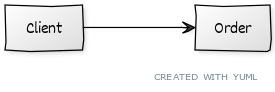
\includegraphics[width=0.6\linewidth]{images/SolidOcpViolationUml}
	\caption{Diagram UML, gdzie \texttt{Client} narusza zasadę OCP.}
	\label{lab1/fig/SolidOcpViolationUml}
\end{figure}
%[Client]->[Order]
%[Client]
%[Order]

Stosując wzorzec projektowy strategia\ref{lab4/sec/strategy}, który zostanie omówiony na kolejnych zajęciach mamy możliwość odwrócenia zależności. Jeśli w~wyniku rozszerzania, zmian funkcjonalności okaże się, że klasa \texttt{Order} powinna zostać zamieniona, będzie można utworzyć nową wersję klasy implementującej interfejs zdefiniowany przez klienta i ją podmienić bez modyfikacji w samej klasie \texttt{Client}.

%Zastosowano interfejs IClient zamiast IOrder, ponieważ związki klas abstrakcyjnych z klasami klienckimi są ściślejsze niż z konkretnymi potomnymi, które je implementują.
\begin{figure}[hbt!]
	\centering
	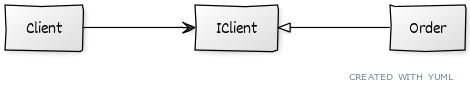
\includegraphics[width=0.9\linewidth]{images/SolidOcpUml}
	\caption{Diagram UML, gdzie \texttt{Client} \textbf{nie} narusza zasady OCP.}
	\label{lab1/fig/SolidOcpUml}
\end{figure}
%[Client]->[IClient]^[Order]
%[Client]
%[IClient]
%[Order]

Wyobraźmy sobie moduł odpowiedzialny za rysowanie figur geometrycznych. Parametrem jednej z~jego metod (\texttt{DrawerShape}) jest kolekcja obiektów. Jeśli w wyniku zmian konieczne okaże się dodanie nowej klasy np. \texttt{Diamond} wymagane będą zmiany w klasie \texttt{Drawer}.
\begin{lstlisting}[caption={Naruszenie zasady OCP}, label={lab1/lst/ocpViolationShapes}]
public class Circle { }
public class Square { }

public static class Drawer 
{
	public static void DrawShapes(IEnumerable<object> shapes) 
	{
		foreach (object shape in shapes) 
		{
			if (shape is Circle) 
			{
				(shape as Circle).DrawCircle();
			} 
			else if (shape is Square) 
			{
				(shape as Square).DrawSquare();
			}
		}
	}
}
\end{lstlisting}

Stosując polimorfizm i abstrakcję możemy uniezależnić klasę \texttt{Drawer} od konkretnych typów. Dzięki utworzeniu wspólnego interfejsu i przekazywanie listy obiektów implementujących ten interfejs, dodanie nowej figury nie będzie wymagało zmian w kodzie klienta. Nie musimy dostosowywać już istniejące kodu do zmian.

\begin{lstlisting}[caption={Poprawne zastosowanie zasady OCP}, label={lab1/lst/ocpShapesCorrect}]
public interface IShape 
{ 
	void Draw(); 
}
public class Circle : IShape { public void Draw() { }}
public class Square : IShape { public void Draw() { } }

public static class Drawer 
{
	public static void DrawShapes(IEnumerable<IShape> shapes) 
	{
		foreach (IShape shape in shapes) 
		{
			shape.Draw();
		}
	}
}
\end{lstlisting}

%Niestety istnieją takie zmiany, na które powyżej pokazana implementacja nie jest odporna np. jeśli kolejność rysowania figur okazałaby się konieczna do uwzględnienia. To projektant musi przewidzieć jakie zmiany są najbardziej prawdopodobne i określić odpowiednie zabezpieczenia. Zamiast stosować punkty szczepień (miejsca w programie, w których przewidujemy, że być może kiedyś będą zmiany), może zastosować zasadę mówiącą, że "Gdy raz mnie oszukasz, powinieneś się wstydzić. Kiedy oszukasz mnie po raz drugi, to ja powinienem się wstydzić". Jednocześnie powinniśmy na bieżąco sprawdzać nasze oprogramowanie i zdobywać wiedzę o prawdopodobnych rodzajach zmian. 

%Problem z kolejnością rysowanych figur możnaby rozwiązać stosując dodatkową klasę ShapeComparer : IComparer, która to zawiera statyczną tablicę priorytetów, na której to podstawie określane są priorytety rysowania figur. Metoda DrawShapes może wtedy wywolać metodę shapes.Sort(new ShapeComparer) prze rysowaniem figur (str. 186).

Oczywiście zmiany będą również konieczne w module, który tworzy instancje obiektów typu \texttt{Shape}. Ale ten proces jest zazwyczaj hermetyzowany w metodzie \texttt{Main} albo w fabrykach\ref{sec/lab2/abstractFactory}.

\subsubsection{Zadanie 2}
Utwórz nowy projekt i dodaj do niego klasę o~nazwie \texttt{UI} z metodą \texttt{Drawer} analogicznie jak zostało to pokazane powyżej\ref{lab1/lst/ocpShapesCorrect}. Utwórz w osobnych plikach klasy: \texttt{Circle}, \texttt{Square}, \texttt{Rectangle} oraz \texttt{Triangle}. Wszystkie powinny implementować interfejs \texttt{IShape} posiadający metodę \texttt{Draw()}. Zaimplementuj w klasach kształtów ten interfejs przez proste wypisywanie na ekranie konsoli informacji, że funkcja \texttt{Draw} została wywołana na przykład w następujący sposób:
\begin{lstlisting}
public class Square : IShape
{
	public void Draw() => Console.WriteLine("Square has been drawn.");
}
\end{lstlisting}
W metodzie \texttt{Main} utwórz kilka instancji klas kształtów i dodaj je do listy albo innego kontenera mogącego przechowywać obiekty implementujące interfejs \texttt{IShape}. Następnie przekaż do metody \texttt{DrawShapes} tę listę (wcześniej utwórz obiekt klasy \texttt{Draw}, aby móc z niej skorzystać).

\subsection{LSP - Zasada podstawienia Liskov (ang. SO\textbf{L}ID)}

Zasada podstawienia Liskov pozawala odpowiedzieć na pytanie jakie są dobre praktyki tworzenia hierarchii klas i co zrobić, aby były one zgodne z zasadą otwarte-zamknięte. Klient powinien móc bez zastanowienia się używać wymiennie klasy bazowej oraz klas pochodnych. W sytuacji braku możliwości podstawienia obiektów pochodnych w miejsce obiektów klasy bazowej występuje naruszenie zasady LSP. Często w konsekwencji zostaje również naruszona zasada OCP.

\begin{myboxWithTitle}{Zasada podstawienia Liskov}
Musi istnieć możliwość zastępowania typów bazowych ich podtypami.
\end{myboxWithTitle}

Lepsze zrozumienie zasady LSP można uzyskać analizując popularny przykład klasy prostokąta oraz klasy kwadratu, która jest pochodną klasy prostokąta. Zasadność stosowania dziedziczenia często jest analizowania przez zadanie sobie pytania czy klasy są w relacji \textbf{IS-A}. Niewątpliwie kwadrat jest prostokątem. Jednak pierwszy problem pojawia się w~sytuacji, gdy chcemy zaimplementować/skorzystać z~właściwości \texttt{Height} i~\texttt{Width} oraz dalej metody \texttt{Area}, zwracającej pole powierzchni danej figury. Właściwości \texttt{Height} i~\texttt{Width} są całkowicie uzasadnione w~przypadku prostokąta, jednak wątpliwe w klasie kwadratu. 

Próbując rozwiązać ten problem można próbować napisać klasę \texttt{Square} tak, że w momencie ustawiania właściwości wysokości albo szerokość w klasie kwadratu, będzie ustawiana zarówno wysokości jak i szerokość na taką samą wartość. Właściwości te mogą w klasie bazowej być wirtualne. Spójrzmy na poniższy kod, w~sytuacji gdy do funkcji zostałby przekazany właśnie taki obiekt kwadratu.
\begin{lstlisting}[caption={Naruszenie zasady LSP}, label={lab1/lst/lspViolationSquareRectangle}]
void Foo(Rectangle r)
{
	r.Width = 5;
	r.Height = 4;
	if(r.Area() != 20) {throw new ...}
}
\end{lstlisting}

Pomimo tego zabiegu klient dalej nie jest w~stanie użyć instancji klasy pochodnej zamiennie w klasą bazową. Najlepszym rozwiązaniem byłoby pominięcie dziedziczenia i napisania klasy \texttt{Sqaure} tak, aby nie dziedziczyła ona po \texttt{Rectangle}.

Przewidzieć takie założenia, można za pomocą  programowanie przez kontrakt (tzw. DBC ang. Design By Contract). Polega ona na dodaniu do metod pewnych warunków wejściowych oraz wyjściowych, które muszą być spełnione, aby metoda mogła się wykonać. 

\begin{mybox}
Ponowna deklaracja procedury (w klasie potomnej) może zastępować warunki wstępne tylko warunkami równymi lub słabszymi, natomiast warunki wyjściowe może zastępować tylko warunkami równymi lub mocniejszymi.
\end{mybox}

Warunki wyjściowe właściwości \texttt{Rectangle.Width} mogłyby zostać zdefiniowane jako:
\begin{lstlisting}
	assert((width == w ) && (height == old.height));
\end{lstlisting}

Innym problemem, może być sytuacja, gdy dana metoda klasy bazowej przyjmuje dowolny obiekt, natomiast w~klasie pochodnej istnieje nieznany wymóg, że obiekt ten musi być konkretnego typu np. z~powodu wykonywania operacji rzutowania. Klasa pochodna będzie zgłaszać niezrozumiały dla klienta wyjątek.

Reguły którymi należy się kierować, aby zachować zgodność z zasadą LSP mogą zostać podzielone na dwie kategorie: warunki kontraktu oraz warunki wariancji. Podczas laboratoriów skupimy się na tych pierwszych. Warunki wariancji natomiast są związane z zmiennością argumentów i typów zwracanych. 
%The concept of type variance in the languages of the Common Language Runtime (CLR) of the Microsoft .NET Framework is limited to generic types and delegates. However, variance in these scenarios is well worth exploring and will equip you with the requisite knowledge to write code that is LSP compliant for variance. This will be explored in depth in the “Covariance and contravariance” section later in this chapter

\subsubsection{Warunki kontraktu}
Warunki wstępne klasy bazowej nie mogą zostać zaostrzone w klasie pochodnej. Warunki końcowe nie mogą zostać złagodzone w klasie pochodnej. Inwarianty muszą pozostać takie same w klasie pochodnej jakie były w~klasie bazowej.

% Często zamienie mówi się, że programiści powinni programować do interfejsów oraz programować do kontraktu. Interfejsy jednak słabo przekazują informację o kontrakcie. Sygantury bardzo niewiele mówią o wymaganiach i gwarancji wywoływanej metody. W językach silnie typowanych jedyne co mamy to informację o typie, ale w tym miejscu intefejsy się kończą i w ich miejsce wchodzą kontrakty. 
% Bardzo wazne jest, aby nazwy argumentow byly opisowe, metody powinny od razu informować co robią, a argumenty czym są. Można nawet w nazwach dodac jednostki miar, aby dodatkowo sprezycoważ argument. 

Sygnatura określona w interfejsie danej metody informuje o tym jakiego typu parametry metoda przyjmuje. Jednak w przypadku, gdy wymagane są dodatkowe ograniczenia np. waga przedmiotu nie może być liczbą ujemną, konieczne jest użycie kontraktu. Warunki początkowe powinny być definiowane tak, aby metoda mogła się wykonać poprawnie. Jednym ze sposobów, aby wymusić stosowanie kontraktu jest rzucenie wyjątkiem, w~przypadku złej wartości argumentu wejściowego. Jeśli kontrakt nie zostanie spełniony, klient będzie zmuszony przechwycić i obsłużyć wyjątek, w przeciwnym razie wykonywanie programu się zakończy.

Warto w tym miejscu powiedzieć, że w przypadku kontraktów należy używać wyjątków, a nie asercji. Asercje służą, do znajdowania naszych błędów, natomiast wyjątki, aby poradzić sobie z błędami popełnionymi przez użytkowników czy innych programistów wykorzystujących nasz kod. Inaczej mówiąc, w przypadku sprawdzania warunków w~publicznym API należy stosować wyjątki. Jeśli sprawdzamy własne, wewnętrzne warunki można używać asercji.

Asercji można używać bardzo liberalnie. Informują one o tym czego kod oczekuje w danym momencie. Wyjątki dotyczą bardziej tego czego żądamy. Dobrze napisane asercje mogą nam powiedzieć nie tylko co się stało oraz gdzie, ale również dlaczego. Służą za dodatkową dokumentację. Jeśli podczas działania programu wystąpi błąd związany z asercją możemy dołączyć debugger do procesu i sprawdzić stan stosu. 
% Asercje z kodu produkcyjnego zostają wycięte może się wydawać, że stosowanie ich nie ma sensu. Jednak jeśli poźniej będzie konieczność odtworzenia problemu przez dewelopera to łatwo będzie możliwość znalezienia źródła problemu.

\subsubsection{Zadanie 3}

Stwórz nowy projekt .NET 5.0.



Utwórz klasę o nazwie \texttt{ShippingStrategy} i dodaj do niej metodę \texttt{CalculateShippingCost}, która będzie przyjmowała argumenty: \texttt{float packageWeigthInKilograms}, \texttt{float packageDimensionXInInches}, \texttt{float packageDimensionYInInches}, \texttt{RegionInfo destination}.

Na górze pliku \texttt{ShippingStrategy} dodaj przestrzeń nazw: \texttt{System.Globalization}, aby móc skorzystać z~\texttt{RegionInfo}:
\begin{lstlisting}
using System.Globalization;
//...
\end{lstlisting}

Wewnątrz metody utwórz zmienną pomocniczą typu \texttt{decimal} i przypisz do niej dowolną wartość (nie ma ona w tym momencie znaczenia). Będzie ona przechowywała zwracaną wartość, nadaj jej stosowną opisową nazwę.

Dodaj do metody kontrakt w postaci rzucanego wyjątku typu \texttt{ArgumentOutOfRangeException} w~przypadku, gdy przekazywane parametry są niewłaściwe np. są liczbami ujemnymi:
\begin{lstlisting}
public decimal CalculateShippingCost(float packageWeightInKilograms, float packageDimensionXInInches, float packageDimensionYInInches, RegionInfo destination)
{
	//Preconditions
	if (packageWeightInKilograms <= 0)
	{
		throw new ArgumentOutOfRangeException(nameof(packageWeightInKilograms), "Package weight can not be negative");
	}
	//...
}
\end{lstlisting}

Na końcu metody zwróć utworzoną wcześniej pomocniczą zmienną.

Analogicznie warunki końcowe powinny być sprawdzane na końcu metody, aby zagwarantować że metoda nie zmieniła stanu obiektu albo, że zwracana wartość jest poprawna. Dodaj warunek końcowy, który będzie sprawdzał, czy obliczone koszty wysyłki są dodatnie. W~przeciwnym razie zgłoś wyjątek.
\begin{lstlisting}
public decimal CalculateShippingCost(float packageWeightInKilograms, float packageDimensionXInInches, float packageDimensionYInInches, RegionInfo destination)
{
	//...
	//Postconditions
     if (shippingCost <= decimal.Zero) throw new ArgumentOutOfRangeException(nameof(shippingCost), "Shipping cost is out of range");
	
	return shippingCost;
}
\end{lstlisting}


W metodzie \texttt{Main} utwórz obiekt klasy \texttt{ShippingStrategy} i wywołaj funkcję z poprawnymi i~błędnymi argumentami, sprawdź czy został wygenerowany wyjątek.

Dodatkowo jeśli klient ma możliwość zmiany pewnej właściwości, która musi przyjmować ściśle określone wartości, powinna ona również zostać zabezpieczona w analogiczny sposób. Jeśli właściwość ta byłaby chroniona, albo prywatna, a jaj wartość byłaby ustawiana w konstruktorze, sprawdzenie należałoby dodać w~konstruktorze klasy.

W utworzonej przed chwilą klasie dodaj prywatną \textbf{zmienna} typu \texttt{decimal} o nazwie \texttt{flatRate}.

Dodaj właściwość \texttt{FlatRate} z metodą dostępu \texttt{get} oraz akcesorem \texttt{set}.

Wewnątrz akcesora \texttt{set} dodaj sprawdzenie ustawianej wartości tak jak dla warunków początkowych i~końcowych.
\begin{lstlisting}
public class ShippingStrategy
{
	private decimal flatRate;
	public decimal FlatRate 
	{ 
		get { return flatRate;}
		set
		{
			//Data invariants
			if (value <= decimal.Zero) throw new ArgumentOutOfRangeException(nameof(value), "Flat rate must be positive and non zero");
			flatRate = value;
		}
	}
	//...
}
\end{lstlisting}
Sprawdź działanie powyższego kontraktu z poziomu klienta - metody \texttt{Main}.


Zamiast umieszczać kod kontraktów wewnątrz metody, lepiej byłoby utworzyć osobne klasy typu \texttt{Weight} czy \texttt{Size} i~to w~nich dodać powyższe kontrakty. Dodaj do projekt klasy pomocnicze \texttt{Size} oraz \texttt{Weight} w~dwóch osobnych plikach:
\begin{lstlisting}
public class Size
{
	public double Height { get; init; }
	public double Width { get; init; }
	
	public Size(double height, double width)
	{
		this.Height = height;
		this.Width = width;
	}
}
\end{lstlisting}
\begin{lstlisting}
public class Weight
{
	public double Value { get; init; }	
	public Weight(double value) => this.Value = value;
}
\end{lstlisting}

W~ten sposób w~całym kodzie kontrakty dla danych typów będą spójne oraz zmniejszy się liczba duplikowanego kodu. Utwórz nowe klasy \texttt{Weight} oraz \texttt{Size} i~umieść w nich właściwości wraz z~zabezpieczeniem przed możliwością ustawienia niepoprawnej wartości. Klasa \texttt{Weight} może posiadać właściwość \texttt{Value}, natomiast \texttt{Size} właściwości \texttt{Height}, \texttt{Width}. Zamień deklarację i ciało metody \texttt{CalculateShippingCost} tak, aby korzystała z~tych klas.

\subsubsection{Zadanie 4}
Zbadaj kontrakty w kontekście zasady LSP:

Oznacz metodę \texttt{CalculateShippingCost} jako wirtualną. Utwórz klasę pochodną klasy \texttt{ShippingStrategy} i nazwij ją np. \texttt{WorldWideShippingStrategy}. Za pomocą słowa kluczowego \texttt{override} przesłoń wirtualną metodę klasy bazowej i~dodaj w~niej sprawdzenie czy wartość argumentu \texttt{destination} jest \texttt{null}. Warunek ten narusza zasadę LSP mówiącą o tym, że nie wolno zaostrzać warunków początkowych. %dotyczy argumentu destination
\begin{lstlisting}
public class WorldWideShippingStrategy : ShippingStrategy
{	
	public override decimal CalculateShippingCost(Weight packageWeightInKilograms, Size packageDimensionInInches, RegionInfo destination)
	{
		//LSP violation
		if (destination == null) throw new ArgumentNullException(nameof(destination), "Destination can not be null or empty");
		//...
	}
}
\end{lstlisting}

Utwórz teraz w metodzie \texttt{Main()} dwa obiekty w sposób pokazany poniżej\ref{lab1/lst/lspShippingStrategiesCall}. 

Zwróć uwagę, że w drugim przypadku został zgłoszony wyjątek. Klient musi w takiej sytuacji rozróżniać różne typu wykorzystywanych obiektów co łamie zasadę LSP oraz wprowadza dodatkowe zależności.  

\begin{lstlisting}[caption={Wywołanie metod klas ShippingStrategy oraz WolrdWideShippingStrategy}, label={lab1/lst/lspShippingStrategiesCall}]
class Program
{
	static void Main(string[] args)
	{
		ShippingStrategy shippingStrategyCustom = new ShippingStrategy();
		ShippingStrategy shippingStrategyWorldWide = new WorldWideShippingStrategy();
		
		var retA = shippingStrategyCustom.CalculateShippingCost(new Weight(10),  new Size(10, 10), null);
		var retB = shippingStrategyWorldWide.CalculateShippingCost(new Weight(10), new Size(10, 10), null);
	}
}
\end{lstlisting}

Analogicznie złamany może być warunek końcowy. Załóżmy, że w klasie bazowej \texttt{ShippingStrategy} tak jak wcześniej koszt wysyłki zawsze jest niezerowy. Natomiast w klasie pochodnej może on być zerowy jeśli, wysyłka jest do tego samego kraju: %dotyczy zmiennej shippingCost
\begin{lstlisting}
public class WorldWideShippingStrategy : ShippingStrategy
{	
	public override decimal CalculateShippingCost(Weight packageWeightInKilograms, Size packageDimensionInInches, RegionInfo destination)
	{
		//...
		//Postconditions LSP violation 
		if (destination == RegionInfo.CurrentRegion)
		{
			shippingCost = decimal.Zero;
		}
	}
}
\end{lstlisting}

Powoduje to ponowne złamanie zasady, że warunki końcowe nie powinny być rozluźniane w klasie pochodnej. Dokładnie ta sama zasada dotyczy wartości niezmiennych (ang. invariant data). W~naszym przykładzie właściwości \texttt{FlatRate}. Klasa pochodna nie powinna w żaden sposób zmieniać nałożonych wcześniej ograniczeń. Aby to sprawdzić dodaj do klasy \texttt{WorldWideShippingStrategy} ponownie właściwość wraz ze słowem kluczowym \texttt{new}:
\begin{lstlisting}
public class WorldWideShippingStrategy : ShippingStrategy
{
	//LSP violation
	public new decimal FlatRate { get; set; }
	//...
}
\end{lstlisting}

Sprawdź powyższe złamania zasady LSP w metodzie \texttt{Main}:
\begin{lstlisting}
class Program
{
	static void Main(string[] args)
	{
		var retC = shippingStrategyWorldWide.CalculateShippingCost(new Weight(10), new Size(10, 10), RegionInfo.CurrentRegion);
		(shippingStrategyWorldWide as WorldWideShippingStrategy).FlatRate = -20;
	}
}
\end{lstlisting}

Aby uprościć tworzenie kontraktów można napisać prostą metodę statyczną, która ułatwi ten proces:
\begin{lstlisting}
public class CustomContract
{
	public static void Requires<TException>( bool Predicate, string Message )
	where TException : Exception, new()
	{
		if ( !Predicate )
		{
			Debug.WriteLine( Message );
			throw new TException();
		}
	}
}  	
\end{lstlisting}

\texttt{Requires} jest metodą generyczną, gdzie \texttt{T} musi być typu referencyjnego oraz posiadać bezparametrowy konstruktor.

% Sytuacja może być niebezpieczne np. jeśli klient przez poczynione założenie, że wartość jest dodania wykona operację dzielenia przez zero.

%\subsubsection{Wykorzystanie kontraktów z \texttt{System.Diagnostics.Contracts}}

%Kontrakty z \texttt{System.Diagnostics.Contracts} nie są już wspierane.

%Jak można było zauważyć pisanie kontraktów w sposób pokazany powyżej może być żmudne. Dodatkowo sprawdzenie naruszenia kontraktu miało miejsce podczas wykonywania się programu. Wykorzystując kontrakty znajdujące się w przestrzeni nazw \texttt{System.Diagnostics.Contracts} można uprościć sobie proces tworzenia kontraktów.
%
%\begin{enumerate}
%	\item Utwórz nowy plik z klasą \texttt{ShippingStrategyCodeContracts}.
%	\item Dodaj na górze pliku przestrzeń nazw za pomocą \texttt{using System.Diagnostics.Contracts}.
%	\item Zamiast wykorzystywać klauzulę \texttt{if} utwórz kontrakt tak jak pokazano poniżej\ref{lab1/lst/lspCodeContractsPreCondition}. Zwróć uwagę, na odwróconą logikę wewnątrz metody \texttt{Requires} względem wcześniejszego przykładu. Dodatkowo istnieje możliwość zdefiniowana zgłaszanego wyjątku.
%	\item Analogicznie można utworzyć kontrakty dla warunków końcowych\ref{lab1/lst/lspCodeContractsPostCondition} oraz danych inwariantnych\ref{lab1/lst/lspCodeContractsDataInvariant}.
%\end{enumerate}

%\begin{lstlisting}[caption={Tworzenie kontraktów z wykorzystaniem \texttt{System.Diagnostics.Contracts} - warunki początkowe}, label={lab1/lst/lspCodeContractsPreCondition}]
%public class ShippingStrategyCodeContracts
%{
%	public virtual decimal CalculateShippingCost(float packageWeightInKilograms, float packageDimensionInInches, string destination)
%	{
%		//Preconditions
%		Contract.Requires(packageWeightInKilograms > 0);
%		Contract.Requires<ArgumentOutOfRangeException>(packageDimensionInInches > 0);
%		
%		//...
%	}
%}
%\end{lstlisting}

%\begin{lstlisting}[caption={Tworzenie kontraktów z wykorzystaniem \texttt{System.Diagnostics.Contracts} - warunki końcowe}, label={lab1/lst/lspCodeContractsPostCondition}]
%public class ShippingStrategyCodeContracts
%{
%	public virtual decimal CalculateShippingCost(float packageWeightInKilograms, float packageDimensionInInches, string destination)
%	{
%		//...
%		
%		//Postconditions
%		Contract.Ensures(Contract.Result<decimal>() > 0);
%		
%		return decimal.MinValue;
%	}
%}
%\end{lstlisting}

%\begin{lstlisting}[caption={Tworzenie kontraktów z wykorzystaniem \texttt{System.Diagnostics.Contracts} - dane inwariantne}, label={lab1/lst/lspCodeContractsDataInvariant}]
%public class ShippingStrategyCodeContracts
%{
%	[ContractInvariantMethod]
%	private void ClassInvariant()
%	{
%		Contract.Invariant(this.FlatRate > 0m, "Flat rate must be positive and non-zero");
%	}   
%	
%	public decimal FlatRate { get; set; }
%}
%\end{lstlisting}
\subsection{ISP - Zasada segregacji interfejsów (ang. SOL\textbf{I}D)}

Interfejsy klas nie powinny być rozbudowane/złożone. Jeżeli jedna klasa korzysta jedynie z~pewnych funkcjonalności jakie zakłada interfejs, a druga z innych to taki interfejs powinien zostać podzielony na dwa niezależne od siebie. Do celów zapewnienia zgodności z zasadą separacji interfejsów można skorzystać z~techniki dziedziczenia wielokrotnego. Należy pamiętać, że w C\# klasa nie może dziedziczyć po więcej niż jeden klasie, natomiast może implementować wiele interfejsów. Obiekty klienckie mogą korzystać z tego samego obiektu za pośrednictwem różnych interfejsów. Powinny one zależeć wyłącznie od wywoływanych przez siebie metod.  

\begin{myboxWithTitle}{Zasada segregacji interfejsów}
Klient nie powinien być zmuszany do zależności od metod, których nie używa.
\end{myboxWithTitle}

Wyobraźmy sobie, że musimy przygotować program obsługujący interfejs użytkownika bankomatu. Konieczne jest zapewnienie możliwości obsługi urządzenia z~wykorzystaniem interfejsu graficznego, syntezatora mowy oraz za pomocą języka Braille'a (klasy interfejsu użytkownika). 

Zakładamy, że każda oęperacja dowolnej transakcji jest realizowana przez osobną klas na przykład mogą to być typy: \texttt{DepositTransaction}, \texttt{WithdrowalTransaction} oraz \texttt{TransferTransaction}, wszystkie mogą dziedziczyć po abstrakcyjnej klasie bazowej \texttt{Transaction} z~pojedynczą metodą \texttt{Execute}. Jednocześnie wszystkie muszą korzystać z klas, które realizują funkcję UI (klasy te powinny implementować interfejs \texttt{IUI}). Klasa realizująca obsługę z wykorzystaniem syntezatora mowy, musi implementować wszystkie możliwe operacje przewidziane przez klasy pochodne względem \texttt{Transaction}, co jest sensowne. Problemem jest jednak fakt, że np. klasa \texttt{DepositTransaction} musi niepotrzebnie znać/posiadać referencje do całego obiektu implementującego UI. Wystarczyłaby by funkcja \texttt{RequestDepositAmount}, obiekt nie jest zainteresowany np. \texttt{RequestTransferAmount}. 

Rozwiązanie tego problemu zostało pokazano na diagramie UML~\ref{lab1/fig/SolidIspUml}. Dzieląc gruby interfejs \texttt{IUI} można odciążyć klientów od posiadania referencji do obiektów, których funkcjonalności nie potrzebują. Co więcej, jeśli zostanie dodana nowa transakcja np. \texttt{PayGasBillTransaction} nie będzie konieczności ponownej przebudowy pozostałych klas transakcji w~wyniku zmiany grubego interfejsu UI. 

\begin{figure}[hbt!]
	\centering
	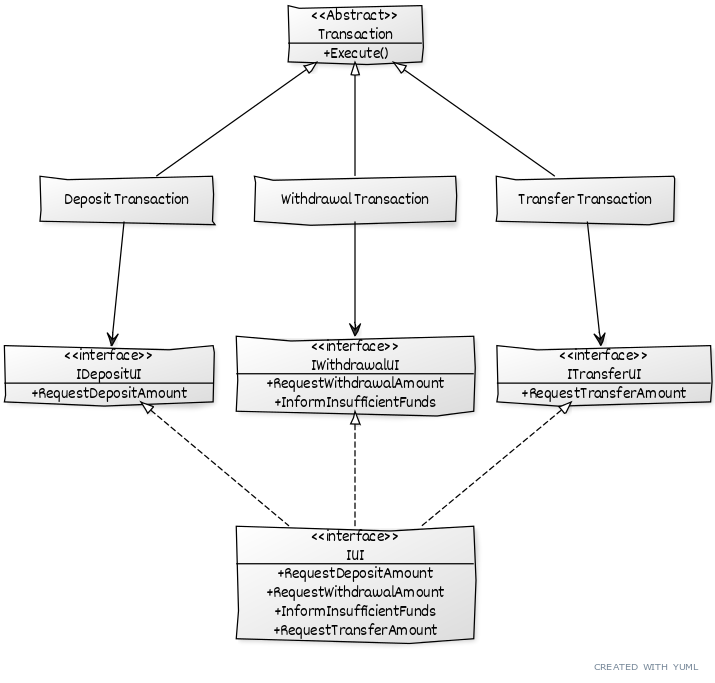
\includegraphics[width=0.8\linewidth]{images/SolidIspUml}
	\caption{Diagram UML projektu w którym zrealizowano zasadę segregacji interfejsów.}
	\label{lab1/fig/SolidIspUml}
\end{figure}
%[Transaction]^[Deposit Transaction]
%[Transaction]^[Withdrawal Transaction]
%[Transaction]^[Transfer Transaction]
%
%[Deposit Transaction]->[DepositUI]
%[Withdrawal Transaction]->[WithdrawalUI]
%[Transfer Transaction]->[TransferUI]
%
%[DepositUI]^-.-[UI]
%[WithdrawalUI]^-.-[UI]
%[TransferUI]^-.-[UI]
%
%[<<Abstract>>Transaction|+Execute()]
%
%[Deposit Transaction]
%[Withdrawal Transaction]
%[Transfer Transaction]
%
%[≪interface≫;DepositUI|+RequestDepositAmount]
%[≪interface≫;WithdrawalUI|+RequestWithdrawalAmount;+InformInsufficientFunds]
%[≪interface≫;TransferUI|+RequestTransferAmount]
%
%[≪interface≫;UI|+RequestDepositAmount;+RequestWithdrawalAmount;+InformInsufficientFunds;+RequestTransferAmount]

W sytuacji, gdy pewna klasa kliencka albo metoda, potrzebowałaby wykorzystać obiekt implementujący zarówno \texttt{IDepositUI} oraz \texttt{IWithdrowalUI}, można jako argumenty konstruktora albo metody przekazać dwa razy ten sam obiekt w następujący sposób: \texttt{Foo(ui,ui)}. Deklaracja konstruktora miałaby postać: \texttt{void Foo(IDepositUI depositUI, IWithdrowalUI withdrowalUi)}.

Ciekawym przykładem zastosowania zasady ISP jest wykorzystanie interfejsów do umożliwienia wykonywania operacji jedynie po wcześniejszym uwierzytelnieniu użytkownika. Przed operacją logowania klient korzysta z~interfejsu \texttt{IUnauthorized}:
\begin{lstlisting}
public interface IUnauthorized
{
	IAuthorized Login(string username, string password);
	void RequestPasswordReminder(string emailAddress);
}
\end{lstlisting}
natomiast po zalogowaniu, poprawnym uwierzytelnieniu, zwracany jest obiekt implementujący \texttt{IAuthorized}:
\begin{lstlisting}
public interface IAuthorized
{
	void ChangePassword(string oldPassword, string newPassword);
	void AddToBasket(Guid itemID);
	void Checkout();
	void Logout();
}
\end{lstlisting}
Drugi z wymienionych interfejsów umożliwia wykonanie większej liczby operacji. Rozwiązanie to zabezpiecza programistę przez udostępnieniem uprzywilejowanych operacji przez niezalogowanego użytkownika. Jest to lepsze rozwiązanie niż umieszczać w interfejsie wszystkie operacje jakie może użytkownik wykonać. 

\subsubsection{Zadanie 5}
Poniższy interfejs\ref{lab1/lst/ispCrudInterface} zawiera zbiór zapytań i poleceń do pamięci trwałej. Dalej natomiast została pokazana przykładowa implementacja\ref{lab1/lst/ispCrudInterfaceImplementation} tego interfejsu korzystająca z bazy danych MongoDB\footnote{Baza danych typu NoSQL w której dane przechowywane są jako pliki z formacie JSON.} do zapytań oraz NHibernate\footnote{Biblioteka ORM przeznaczone na platformę .NET do mapowania obiektów modelu domeny na relacyjną bazę danych.} do poleceń.
\begin{lstlisting}[caption={Interfejs zawierający zbiór operacji CRUD}, label={lab1/lst/ispCrudInterface}]
public interface IPersistence
{
	IEnumerable<Entity> GetAll();
	Entity GetByID(Guid identity);
	IEnumerable<Entity> FindByCriteria(string criteria);
	void Save(Entity entity);
	void Delete(Entity entity);
}
\end{lstlisting}

\begin{lstlisting}[caption={Implementacja interfejsu \texttt{IPersistence}}, label={lab1/lst/ispCrudInterfaceImplementation}]
public class Persistence : IPersistence
{
	private readonly ISession session;
	private readonly MongoDatabase mongo;
	public Persistence(ISession session, MongoDatabase mongo)
	{
		this.session = session;
		this.mongo = mongo;
	}
	public IEnumerable<Entity> GetAll()
	{
		return mongo.GetCollection<Entity>("entities").FindAll();
	}
	public Entity GetByID(Guid identity)
	{
		return mongo.GetCollection<Entity>
		("entities").FindOneById(identity.ToBson());
	}
	public IEnumerable<Entity> FindByCriteria(string criteria)
	{
		var query = BsonSerializer.Deserialize<QueryDocument>
		(criteria);
		return mongo.GetCollection<Entity>("entities").Find(query);
	}
	public void Save(Entity entity)
	{
		using(var transaction = session.BeginTransaction())
		{
			session.Save(entity);
			transaction.Commit();
		}
	}
	public void Delete(Entity entity)
	{
		using(var transaction = session.BeginTransaction())
		{
			session.Delete(entity);
			transaction.Commit();
		}
	}
}
\end{lstlisting}
Często można natomiast się spotkać z rozdzieleniem operacji odczytu i aktualizacji bazy danych. Przykładem tej koncepcji jest m.in wzorzec CQRS, o którym szerzej będziemy mówić przy okazji czynnościowych wzorców projektowych~\ref{sec/lab4/cqrs}. Na ten moment najprościej ujmując polega on na rozdzieleniu operacji odczytu od operacji aktualizacji, dodawania i~usuwania z/do bazy danych.

Zastanów się jak można podzielić interfejs\ref{lab1/lst/ispCrudInterface} na dwa mniejsze: jeden dla poleceń, drugi dla zapytań. Dwie klasy np. \texttt{CommandsNHibernate} oraz \texttt{QueriesMongo} mogłyby implementować odpowiednio \texttt{ICommands} i~\texttt{IQueries}. Klasa kontrolera w takiej sytuacji mogłaby posiadać referencję do dwóch obiektów implementujących wspomniane interfejsy. Takie podejście pozwala na niezależne korzystanie z dwóch rodzajów baz danych, ich swobodną wymianę i skalowanie. Implementacje mogłyby znajdować się różnych w pakietach co jest dodatkową korzyścią 

Utwórz nowy projekt .NET 5.0 i~zaproponuj rozdzielenie powyższego interfejsu\ref{lab1/lst/ispCrudInterface} w~sposób wyżej opisany. Aby wyeliminować błędy kompilacji, konieczne będzie dodanie dwóch pakietów NuGet. W tym celu PPM kliknij na nazwę projektu i wybierz opcję Manage NuGet Packages. Następnie znajdź i zainstaluj pakiet \texttt{mongocsharpdriver} oraz \texttt{NHibernate}. Dodatkowo utwórz pustą klasę \texttt{Enitity}:
\begin{lstlisting}
public class Entity {}
\end{lstlisting}
%\begin{lstlisting}
%public interface IQueries
%{
%	IEnumerable<Item> GetAll();
%	Item GetByID(Guid identity);
%	IEnumerable<Item> FindByCriteria(string criteria);
%}
%// . . .
%public interface ICommands
%{
%	void Save(Item item);
%	void Delete(Item item);
%}
%\end{lstlisting}
%
%\begin{lstlisting}
%public class QueriesMongo : IQueries
%{
%	private readonly MongoDatabase mongo;
%	public QueriesMongo(MongoDatabase mongo) =>	this.mongo = mongo;
%	public IEnumerable<Item> GetAll()
%	{
%		return mongo.GetCollection<Item>("items").FindAll();
%	}
%	public Item GetByID(Guid identity)
%	{
%		return mongo.GetCollection<Item>
%		("items").FindOneById(identity.ToBson());
%	}
%	public IEnumerable<Item> FindByCriteria(string criteria)
%	{
%		var query = BsonSerializer.Deserialize<QueryDocument>
%		(criteria);
%		return mongo.GetCollection<Item>("Items").Find(query);
%	}
%}
%\end{lstlisting}
%
%\begin{lstlisting}
%public class CommandsNHibernate : ICommands
%{
%	private readonly ISession session;
%	public CommandsNHibernate(ISession session) => this.session = session;
%	public void Save(Item item)
%	{
%		using(var transaction = session.BeginTransaction())
%		{
%			session.Save(item);
%			transaction.Commit();
%		}
%	}
%	public void Delete(Item item)
%	{
%		using(var transaction = session.BeginTransaction())
%		{
%			session.Delete(item);
%			transaction.Commit();
%		}
%	}
%}
%\end{lstlisting}


\subsection{DIP - Zasada odwracania zależności (ang. SOLI\textbf{D})}\label{lab1/sec/dip}

Głównie za sposób działania aplikacji odpowiadają moduły wysokopoziomowe. To one zawierają logikę biznesową, która często jest wielokrotnie wykorzystywana. Przemyślana architektura obiektowa powinna składać się z wyraźnie zdefiniowanych i odznaczających się warstw. Usługi powinny być opisane odpowiednimi, niezmiennymi interfejsami\footnote{Rzadko udaje się osiągnąć sytuację, w której interfejsy są niezmienne w szczególności na początkowym etapie projektu. Jednak powinny one być zdecydowanie bardziej stabilne niż klasy.}.

\begin{myboxWithTitle}{Zasada odwracania zależności}
	A. Moduły wysokopoziomowe nie powinny zależeć od modułów niskopoziomowych. Obie grupy modułów powinny zależeć od abstrakcji.\\
	B. Abstrakcje nie powinny zależeć od szczegółowych rozwiązań. To szczegółowe rozwiązania powinny zależeć od abstrakcji.
\end{myboxWithTitle}

Nie należy postrzegać bibliotek jako właścicieli interfejsów. Interfejsy powinny być powiązane ze swoimi właścicielami i to klasy z innej warstwy powinny implementować te interfejsy. % Lekki wstep o Clean Architecture Taylor'a i o tym jak interfejs opisujacy dostep do bazy danych znajduje sie w warstwie Application, natomiast implementacja w Infrastructure.
Pozwala to tworzyć oprogramowanie, które jest elastyczne. Jeśli dany zestaw jest wykorzystywany przez kilku klientów np. pobrany pakiet NuGet to warto stworzyć dodatkową warstwę abstrakcji, która umożliwi w~przyszłości zmianę tego pakietu, bez konieczności wprowadzania zmian po stronie klienta. Można to osiągnąć np. stosując wzorzec projektowy Adapter~\ref{sec/lab3/adapter}, który zostanie omówiony na przyszłych zajęciach. Oczywiście jeśli mamy do czynienia z klasami, które są zmieniane bardzo rzadko, albo mamy wysoki poziom zaufania to autorów to uzależnienie się od nich nie jest czymś złym. Ciężko znaleźć sens, tworzenia dodatkowej warstwy pośredniej do komunikowania się np. z~klasą \texttt{string}.

Jako przykład zastosowania zasady DIP wyobraźmy sobie dwie klasy \texttt{Button} oraz \texttt{Lamp}. Klasa przycisku ma możliwość sterowania lampą. W~najprostszej, naiwnej implementacji można by dodać pole w klasie \texttt{Button} przechowujące referencje do obiektu lampy. \texttt{Lamp} mógłby być przekazywany np. jako argument konstruktora. Dlaczego te podejście jest złe i łamie zasadę DIP? \texttt{Button} będący wysokopoziomową abstrakcją, jest uzależniony od niskopoziomowego obiektu lampy.

Powyższy problem można rozwiązać przez dodanie interfejsu np. \texttt{ISwitchableDevice} i~wstrzykiwanie obiektu go implementującego do obiektu \texttt{Button}. Teraz wystarczy, aby \texttt{Lamp} implementował ten interfejs. W~przypadku, kiedy przycisk będzie miał zostać wykorzystany do sterowania np. silnikiem albo piecem wystarczy utworzyć nowy obiekt \texttt{Motor} albo \texttt{Heater}, który będzie implementował \texttt{ISwitchableDevice} i~przekazać go do obiektu \texttt{Button}.

Na poniższym diagramie UML\ref{lab1/fig/DipUml} pokazano hierarchię klas zgodną z zasadą odwracania zależności. W~tym przypadku interfejsy i implementacje zostały umieszczone w osobnych zestawach. Klienci posiadają referencje jedynie do zestawów z interfejsami. W~idealnym scenariuszu interfejsy nie powinny posiadać żadnych zależności, kod kliencki również. To implementacje powinny zależeć od interfejsów. Klasy zestawu \texttt{Controllers} nie są związane z klasami zestawu \texttt{ServicesImplementations}, a jedynie z abstrakcją w postaci interfejsów zestawu \texttt{ServiceInterfaces}. Analogicznie sytuacja wygląda w przypadku zależności zestawu \texttt{ServicesImplementations} od \texttt{Domain}. Warto zauważyć, że od szczegółu jakim jest wykorzystywany ORM (ang. Object-Relational Mapping)\footnote{Technika, która pozwala na zapytania i polecenia do bazy danych z wykorzystaniem paradygmatów programowania obiektowego. Zazwyczaj pisząc ORM mamy na myśli bibliotekę, która implementuje technikę ORM. Pozwala nam na uniezależnienie się od konkretnej bazy danych, komunikacją z nią odbywa się za pomocą konkretnej biblioteki ORM np. NHiberante czy EntityFramework.} nie zależy żaden moduł wyższego poziomu. Powoduje to, że zmiana tego komponentu nie pociągnie za sobą zmian w kodzie warstw wyższych i nie będzie wymagała ich ponownej kompilacji. 
%klienci jako klasy, ktore korzystaja z obiektow innych klas, a nie metoda Main. Oczywiscie klasa/kontener IoC musi posiadac referencej, aby moc utworzy dane instancje.
\begin{figure}[hbt!]
	\centering
	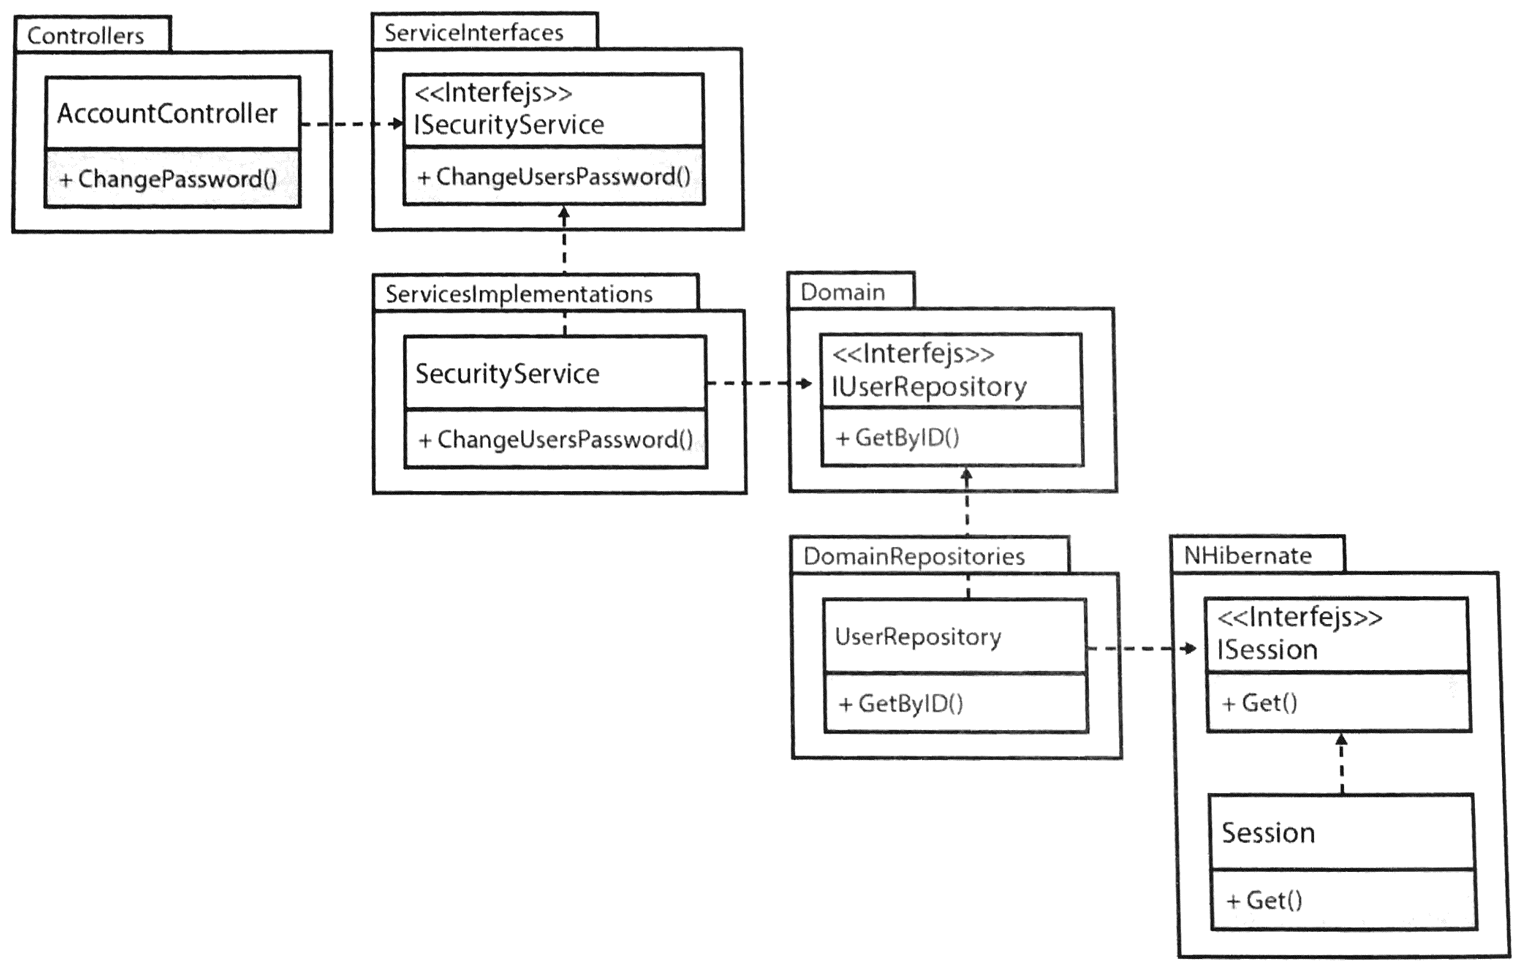
\includegraphics[width=0.9\linewidth]{images/SolidDip}
	\caption{Diagram UML hierarchii klas zgodnej z regułą DIP\cite{adaptatywny_kod_hall}}
	\label{lab1/fig/DipUml}
\end{figure}

\subsubsection{Zadanie 6}
Przeanalizuj poniższy kod i zmień go tak, aby był zgodny z omawianą zasadą DIP.
\begin{lstlisting}
public class Regulator
{
	const byte THERMOMETER = 0X86;
	const byte FURNACE = 0X87;
	const byte ENGAGE = 1;
	const byte DISENGAGE = 0;
	
	void Regulate(double minTemp, double maxTemp)
	{
		for (; ; )
		{
			while (this.Read(THERMOMETER) > minTemp)
			{
				Thread.Sleep(1000);
			}
			this.Write(FURNACE, ENGAGE);
			while (this.Read(THERMOMETER) < maxTemp)
			{
				Thread.Sleep(1000);
			}
			this.Write(FURNACE, DISENGAGE);
		}
	}
	
	byte Read(byte register)
	{
		return 0x00; //returned value not relevant.
	}
	void Write(byte register, byte value)
	{
		//...
	}
}
\end{lstlisting}
% engage - zalaczac, furnace - piec 
% In physics and materials science, the Curie temperature (TC), or Curie point, is the temperature above which certain materials lose their permanent magnetic properties. The Curie temperature is named after Pierre Curie, who showed that magnetism was lost at a critical temperature.[1]. Curie point electro-magnets have been proposed and tested for actuation mechanisms in passive safety systems of fast breeder reactors, where control rods are dropped into the reactor core if the actuation mechanism heats up beyond the material's curie point. Other uses include temperature control in soldering irons.

Możesz utworzyć dwa dodatkowe projekty jeden w którym dodasz interfejsy, jeden dla obiektów mierzących temperaturę \texttt{ISensor} i jeden dla obiektów odpowiedzialnych za zmianę temperatury np. pieców \texttt{IDevice}. Natomiast drugi projekt niech zawiera implementacje utworzonych przed chwilą interfejsów np. \texttt{Thermometer} oraz \texttt{Heater}. Klasa \texttt{Regulator} powinna następnie zostać uzależniona od projektu z interfejsami. Obiekty implementujące \texttt{ISensor} oraz \texttt{IDevice} powinny zostać wstrzyknięte do klasy przez konstruktor. W metodzie \texttt{main} utwórz instancję klasy \texttt{Regulator} i sprawdź jej działanie wywołując metodę \texttt{Regulate()}.

\subsection{Kontenery IoC (ang. Inversion of Control)}
Kontenery IoC takie jak Castle Windsor, Autofac czy Ninject ułatwiają wstrzykiwanie zależności. Jeśli pracujemy nad dużym projektem, w którym klasy zależą od wielu innych i wykorzystują mechanizm wstrzykiwania zależności można wykorzystać kontener IoC, aby ułatwić sobie proces tworzenia obiektów. 

Na przykład tworzenie obiektu \texttt{CustomerService} pokazanego poniżej\ref{lab1/lst/dpiComplexObjectConstruction} wymaga utworzeniu wielu innych obiektów i przekazania ich jako argumenty konstruktora.
\begin{lstlisting}[caption={Tworzenie obiektu posiadającego zależności wstrzykiwane przez konstruktor }, label={lab1/lst/dpiComplexObjectConstruction}]
public CustomerData GetCustomerData(string customerNumber)
{
	var customerApiEndpoint = ConfigurationManager.AppSettings["customerApi:customerApiEndpoint"];
	var logFilePath = ConfigurationManager.AppSettings["logwriter:logFilePath"];
	var authConnectionString = ConfigurationManager.ConnectionStrings["authorization"].ConnectionString;
	using(var logWriter = new LogWriter(logFilePath ))
	{
		using(var customerApiClient = new CustomerApiClient(customerApiEndpoint))
		{
			var customerService = new CustomerService(
			new SqlAuthorizationRepository(authorizationConnectionString, logWriter),
			new CustomerDataRepository(customerApiClient, logWriter),
			logWriter
			);   
			
			return customerService.GetCustomerData(string customerNumber);
		}
	}
}
\end{lstlisting}
Wykorzystując kontener IoC można zarejestrować zależności, które będą tworzone i wstrzykiwane automatycznie. Jeśli dana klasa potrzebuje np. obiektu implementującego \texttt{ILogWriter}, kontener utworzy odpowiednią instancję pod warunkiem, że została ona wcześniej zarejestrowana. Jeżeli np. tym obiektem jest \texttt{LogWriter} i wymaga on ścieżki do pliku, można również taką ścieżkę zarejestrować jako wartość klucza w~\texttt{AppSettings}. Kontener ,,wie'' jakie obiekty, jakich typów muszą być utworzone i wstrzyknięte, aby spełnić wymagania tworzonej klasy. Jeśli odpowiedni obiekt nie został wcześniej zarejestrowany to zostanie zgłoszony wyjątek o~tym informujący. Dodatkowo kontenery umożliwiają sprecyzowanie czy jedna i ta sama instancja ma zostać przekazana do wszystkich obiektów, które jej potrzebuje czy np. za każdym razem powinien być tworzony nowy obiekt.

Kontenery IoC powinny być wykorzystywane jedynie do wiązania poszczególnych elementów programu. Jeśli chcemy tworzyć obiekty podczas działania programu należy wykorzystywać fabryki\ref{sec/lab2/abstractFactory}. Trzeba unikać sytuacji w~których w~całym programie znajdują się referencje do kontenera. Zazwyczaj wystarcza jedno pobranie obiektu np. typu \texttt{Application}, natomiast reszta powiązań powinna odbywać się po stronie kontenera IoC.

\subsubsection{Zadanie 7}\label{lab1/ex/IoC}
Utwórz dwa projekty w solucji. Jeden niech będzie biblioteką, drugi natomiast aplikacją konsolową. Dodaj referencję do biblioteki w aplikacji konsolowej. Aby to zrobić kliknij PPM na projekt aplikacji konsolowej, dalej \texttt{Add} i \texttt{Project Reference...}, następnie wskaż odpowiedni zestaw. W~projekcie biblioteki utwórz następującą hierarchię klas pokazaną na rysunku\ref{lab1/fig/IoC}.
\begin{figure}[hbt!]
	\centering
	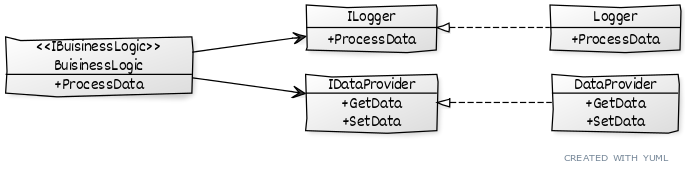
\includegraphics[width=0.8\linewidth]{images/ExerciseIocLib}
	\caption{Diagram UML hierarchii klas biblioteki z zadania~\ref{lab1/ex/IoC}}
	\label{lab1/fig/IoC}
\end{figure}

%[BuisinessLogic]->[ILogger]
%[BuisinessLogic]->[IDataProvider]
%[ILogger]^-.-[Logger]
%[IDataProvider]^-.-[DataProvider]
%
%[≪IBuisinessLogic≫;BuisinessLogic|+ProcessData]
%[ILogger|+ProcessData]
%[Logger|+ProcessData]
%[IDataProvider|+GetData;+SetData]
%[DataProvider|+GetData;+SetData]

Zaimplementuj metody tak, aby wypisywały informację na konsoli o tym jaka metoda jest aktualnie wykonywana np.:
\begin{lstlisting}
public class DataProvider : IDataProvider
{
	public void GetData() => Console.WriteLine("Data downloading...");
	public void SetData() => Console.WriteLine("Data saving...");
}
\end{lstlisting}

Dodaj za pomocą menadżera pakietów NuGet pakiet \texttt{Autofac} do projektu aplikacji konsolowej.
Następnie utwórz w osobnym pliku klasę w której będzie następowała konfiguracja kontenera:
\begin{lstlisting}[caption={Konfiguracja kontenera IoC}, label={lab1/lst/autofacContainterConfig}]
public static class ContainerConfig
{
	public static IContainer Configure()
	{
		var builder = new ContainerBuilder();
		
		//...
		
		return builder.Build();
	}
}
\end{lstlisting}
Aby móc ,,pobrać'' instancję danej klasy z kontenera w pierwszej kolejności należy skojarzyć dane klasy z~odpowiadającymi im interfejsami. Inaczej mówiąc konieczne jest przekazanie informacji jaką klasę chcemy wykorzystać w miejsce danej abstrakcji. Należy to zrobić w następujący sposób:
\begin{lstlisting}
builder.RegisterType<BusinessLogic>().As<IBusinessLogic>();
//...
\end{lstlisting}
Powyższy fragment kodu oraz pozostałe rejestracje umieść w metodzie \texttt{Configure} klasy \texttt{ContainerConfig} \ref{lab1/lst/autofacContainterConfig}.

Do projektu aplikacji konsolowej dodaj również interfejs \texttt{IApplication}, z jedną metodą \texttt{Run()} nie zwracającą żadnego obiektu. W pliku \texttt{Application} umieść implementację interfejsu \texttt{IApplication}:
\begin{lstlisting}
public class Application : IApplication
{
	private readonly IBusinessLogic businessLogic;	
	public Application(IBusinessLogic businessLogic) => this.businessLogic = businessLogic;	
	public void Run() => businessLogic.ProcessData();
}
\end{lstlisting}

W metodzie \texttt{Main} umieść poniższy kod:
\begin{lstlisting}
static void Main(string[] args)
{
	//First thing we want to in program do is wireup the container and dependencies
	var container = ContainerConfig.Configure();
	
	using(var scope = container.BeginLifetimeScope()) //new scope 
	{
		var app = scope.Resolve<IApplication>(); //we need IApplication object, hence container gives us one
		app.Run();
	}
	
	Console.ReadLine();
}
\end{lstlisting}
Uruchom program i sprawdź, czy kontener poprawnie powiązał i stworzył wszystkie obiekty.

W momencie wywołania \texttt{Resolve} kontener sprawdza jakiego typu obiekty należy przekazać do konstruktora obiektu i wstrzykuje je za nas. W naszym przypadku po wywołaniu metody \texttt{Resolve<IApplication>} kontener ,,widzi'', że wymagany jest obiekt implementujący \texttt{IBusinessLogic}, aby utworzyć \texttt{Application}. Dalej \texttt{BusinessLogic} wymaga przekazania obiektu implementującego \texttt{ILogger} oraz \texttt{IDataProvider}. I~w~tym przypadku zostaną za nas utworzone odpowiednie obiekty i przekazane do \texttt{BusinessLogic} tak, aby mógł on zostać stworzony na potrzeby \texttt{Application}.

Aby ułatwić proces wiązania danych obiektów, można zamiast rejestrować poszczególne typy, zarejestrować cały zestaw wraz z określeniem pewnych warunków. Można na przykład zarejestrować wszystkie obiekty z~zestawu, których nazwy zaczynają się danym prefiksem, albo znajdują się w danym folderze. Można również powiązać wszystkie klasy z zestawu z odpowiadającymi im interfejsami.
\begin{lstlisting}
builder.RegisterAssemblyTypes(Assembly.Load(nameof(DependencyInversionPrincipleLib)))
//.Where(t => t.Namespace.Contains("Loggers")) //only from specific folder
.AsImplementedInterfaces(); //register the type as providing all of its public interfaces as services (excluding IDisposable).
\end{lstlisting}

% Jeśli zarejestrujemy kilka implementacji tego samego interfejsu, to Autofac utworzy jeden typ \texttt{IEnumerable<IInterface>}. Dalej taka kolekcja jest wstrzykiwana podczas tworzenia obiektu. 
% Inaczej można wykorzystać konkretną implementację na trzy sposobu:
% - typy wyliczeniowe,
% - metadane z Autofac
% - metadane w kazdym widoku
% Typy wyliczeniowe:
%\begin{lstlisting}
%public enum ViewerType { PdfLarge, PdfSmall, XlsLarge, XlsSmall }
%builder.RegisterType<PdfViewerLarge>().Keyed<IViewer>(ViewerType.PdfLarge);
%builder.RegisterType<PdfViewerSmall>().Keyed<IViewer>(ViewerType.PdfSmall);
%builder.RegisterType<XlsViewerLarge>().Keyed<IViewer>(ViewerType.XlsLarge);
%
%
%public class HomeController : Controller
%{
%	private readonly IIndex<ViewerType, IViewer> _viewers;
%	
%	public HomeController(IIndex<ViewerType, IViewer> viewers)
%	{
%		_viewers = viewers;
%	}
%}
%
%public ActionResult Index()
%{
%	var viewer = _viewers[ViewerType.PdfLarge];
%	
%	// do something with viewer
%	
%	return View();
%}
%\end{lstlisting}
% 
%Można również dodać metadane to rejestrowanego typu.
%
%\begin{lstlisting}
%builder.Register(c => new PdfViewerLarge())
%.As<IViewer>()
%.WithMetadata("FileType", ".pdf");
%\end{lstlisting}
% Metadane z autofac:
%Można również użyć metadanych silnie typowanych. Wcześniej konieczne jest określenie kluczy metadanych.
%
%\begin{lstlisting}
%public interface IViewerMetadata
%{
%	string FileType { get; }
%	long MaxFileSize { get; }
%}
%\end{lstlisting}
%
%Dalej już można wykorzystywać tych  metadanych.
%
%\begin{lstlisting}
%builder.RegisterType<XlsViewerSmall>()
%.As<IViewer>()
%.WithMetadata<IViewerMetadata>(m =>
%{
%	m.For(p => p.MaxFileSize, 10000);
%	m.For(p => p.FileType, ".xls");
%});
%\end{lstlisting}
%
%W kontrolerze MVC widoki będą wstrzykiwane w następujący sposób:
%
%\begin{lstlisting}
%public class HomeController : Controller
%{
%	private IEnumerable<Meta<IViewer, IViewerMetadata>> _viewers;
%	
%	public HomeController(
%	IEnumerable<Meta<IViewer, IViewerMetadata>> viewers)
%	{
%		_viewers = viewers;
%	}
%}
%\end{lstlisting}
%
%Na koniec można już wykorzystywać konkretną implementację.
%
%\begin{lstlisting}
%public ActionResult Index()
%{
%	var viewer = _viewers.Single(
%	it => it.Metadata.FileType == ".xls" &&
%	it.Metadata.MaxFileSize > 1000
%	).Value;
%	
%	
%	// do something with viewer
%	
%	return View();
%}
%\end{lstlisting}
\clearpage
\section{Wzorce projektowe (1) - konstrukcyjne}
\url{https://softwareengineering.stackexchange.com/questions/365119/is-using-new-in-the-constructor-always-bad}
Wzorce kreacyjne pozwalają na tworzenie obiektów w sposób zwiększający elastyczność. Zamiast tworzyć obiekty w wielu miejscach w programie, zadaniem konstrukcji nowych instancji można obciążyć osobne klasy. Użycie słowa kluczowego \texttt{new} narusza omawianą wcześniej zasadę odwracania zależności, powodując trudności z testowaniem kodu i zmniejszając jego elastyczność. 

\subsection{Fabryka abstrakcyjna (ang. abstract factory)}
Fabryka abstrakcyjna jest wzorcem projektowym, który przenosi proces tworzenia obiektów (często ze sobą w jakiś sposób powiązany) do osobnej klasy implementującej interfejs zawierający listę metod tworzących dane obiekty. Co więcej tworzone przez fabryki instancje również powinny posiadać zgodne interfejsy.

Klient może posiadać konstruktor, który jako parametr przyjmie obiekt implementujący interfejs abstrakcyjny. Wewnątrz konstruktora klient wywołując odpowiednie metody może tworzyć konkretne obiekty bez znajomości ich szczegółowej implementacji. Przekazując inny obiekt fabryki abstrakcyjnej możliwa jest łatwa zmiana wykorzystywanych przez klienta obiektów.  

Przykład:
Aplikacja wykorzystująca interfejs graficzny mogłaby przyjmować jako argument obiekty fabryki implementujące interfejs \texttt{IGuiFactory}. Interfejs ten mógłby definiować metody tworzenia poszczególnych elementów graficznych np. \texttt{createButton()}, \texttt{createListBox()}, \texttt{createProgressBar()} itp. Następnie w zależności od systemu operacyjnego można by stworzyć obiekty fabryk \texttt{WindowsFactory} oraz \texttt{UnixFactory}, oba implementujące określony wcześniej interfejs. Aplikacja posiadające logikę rysująca okno użytkownika nie musi w takim przypadku nawet wiedzieć z jakim systemem ma do czynienia, jest od niego niezależna. Może wywoływać metody tworzące kontrolki UI za pomocą abstrakcyjnego interfejsu \texttt{IGuiFactory}. Wybór konkretnej fabryki mógłby być określany w momencie uruchamiania się aplikacji.



\begin{figure}[hbt!]
	\centering
	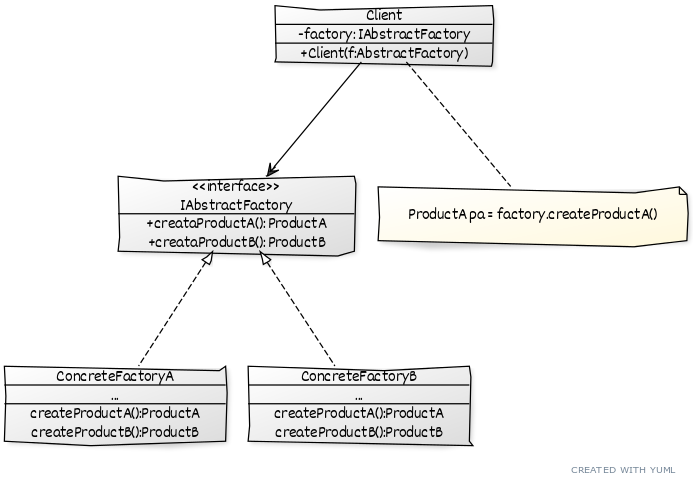
\includegraphics[width=0.9\linewidth]{images/AbstractFactoryUml}
	\caption{Diagram UML wzorca Fabryka Abstrakcyjna.}
	\label{lab2/fig/AbstractFactoryUml}
\end{figure}
%[Client]->[IAbstractFactory]
%[Client]-[note: ProductA pa = factory.createProductA(){bg:cornsilk}]
%[IAbstractFactory]^-.-[ConcreteFactoryA]
%[IAbstractFactory]^-.-[ConcreteFactoryB]
%
%[≪interface≫;IAbstractFactory|+creataProductA(): ProductA;+creataProductB(): ProductB;]
%[Client|-factory: IAbstractFactory|+Client(f:AbstractFactory);]
%[ConcreteFactoryA|...|createProductA():ProductA;createProductB():ProductB]
%[ConcreteFactoryB|...|createProductA():ProductA;createProductB():ProductB]


\subsection{Budowniczny (ang. builder)}
Budowniczy jest wzorcem, który może być wykorzystany do tworzenia złożonego obiektu krok po kroku. Czasami istnieje pokusa stworzenia konstruktora przyjmującego dużą liczbę argumentów np. dana klasa korzysta z wielu zależności albo niektóre jej cechy mogą być parametryzowane. Część z tych argumentów może w ogóle nie być konieczna. Budowniczy przenosi proces tworzenia takiej instancji do osobnego obiektu. 

Czynności wywoływania poszczególnych metod można przenieść do osobnego obiektu kierownika (ang. director), który będzie przyjmował jako argument konstruktora obiekt budowniczego i wywoływał metody interfejsu \texttt{IBuilder}.

Konkretni budowniczowie powinni dostarczyć swoje własne metody zwracania wyników procesu budowania obiektu. Różni budowniczowie mogą zwracać zupełnie inne typy dlatego tego procesu często nie da się umieścić w interfejsie \texttt{IBuilder} (przynajmniej w przypadku języków programowania, które są silnie typowane). 
 
Wzorzec budowniczy często wspiera tzw. płynne interfejsy (ang. Fluent Interface). Z przykładem użycia tego mechanizmu można się spotkać w zapytaniach LINQ, gdzie zamiast wywoływać kolejne metody progresywnie (w kolejnych wierszach), można je wywoływać kaskadowo po kropce.

\begin{lstlisting}[caption={Wykorzystanie płynnych interfejsów w zapytania LINQ}, label={lab2/lst/fluentInterfaceLinq}]
var translations = new Dictionary<string, string>
{
	{"cat", "chat"},
	{"dog", "chien"},
	{"fish", "poisson"},
	{"bird", "oiseau"}
};

// Find translations for English words containing the letter "a",
// sorted by length and displayed in uppercase
IEnumerable<string> query = translations
.Where   (t => t.Key.Contains("a"))
.OrderBy (t => t.Value.Length)
.Select  (t => t.Value.ToUpper());

// The same query constructed progressively:
var filtered   = translations.Where (t => t.Key.Contains("a"));
var sorted     = filtered.OrderBy   (t => t.Value.Length);
var finalQuery = sorted.Select      (t => t.Value.ToUpper());
\end{lstlisting}

W przeciwieństwie do wzorca fabryki abstrakcyjnej, która tworzy obiekty (często ze sobą powiązane) w jednym kroku, budowniczy tworzy jeden złożony obiekt krok po kroku.
\clearpage
%\section{Wzroce projektowe (2) - strukturalne}

Strukturalne wzorce projektowe wyjaśniają jak łączyć obiekty i klasy w większe struktury zachowując jednocześnie prostotę i elastyczność.

\subsection{Adapter (ang. adapter)}\label{sec/lab3/adapter}

Wzorzec który pozwala na działanie dwóch komponentów o niezgodnych interfejsach nazywany jest Adapterem. Jeśli klasa potrzebuje do działania obiektu klasy o określonym interfejsie, natomiast klasa która mogłaby zostać wykorzystana posiada inny, niezgodny interfejs, można utworzyć klasę adaptera, która dostosuje niezgodne interfejsy. Stosuje się go do dopasowywania kodu, który już istnieje. Jest często wykorzystywany w~celu wykorzystania zewnętrznego zestawu firm trzecich np. pobranego z menadżera pakietów NuGet, którego interfejs jest niezgodny z tym używanym w naszej aplikacji.

\begin{figure}[hbt!]
	\centering
	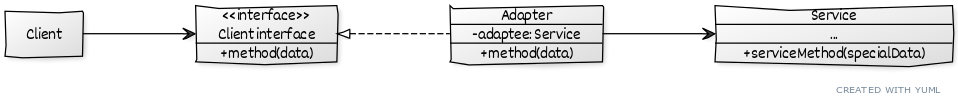
\includegraphics[width=0.9\linewidth]{images/AdapterUml}
	\caption{Diagram UML wzorca Adapter.}
	\label{lab3/fig/AdapterUml}
\end{figure}
%[Client interface]^-.-[Adapter]
%[Adapter]->[Service]
%[Client]->[Client interface]
%
%[Client]
%[<<interface>>Client interface|+method(data)]
%[Adapter|-adaptee: Service|+method(data)]
%[Service|...|+serviceMethod(specialData)]

Wyobraźmy sobie sytuację, w której mamy działający komponent i do logowania informacji o swoim działaniu wykorzystuje napisany przez nas zestaw np. bibliotekę. Klasa logera implementuje określony interfejs np. \texttt{ILogger}. Wykorzystując ten interfejs, klasa kliencka używa obiektu klasy logera do logowania. Jeśli za jakiś czas okaże się konieczne wykorzystanie bardziej rozbudowanego narzędzia do logowania np. pakietu NLog, możemy albo zmieniać odwołania w kodzie klienckim, albo wykorzystać wzorzec Adapter. W drugim przypadku adapterem będzie klasa implementująca nasz interfejs \texttt{ILogger} i posiadająca obiekt typu \texttt{NLog.Logger} przekazany/wstrzyknięty np. jako argument konstruktora. Wszystkie metody interfejsu \texttt{ILogger} są przekazywane do odpowiednich metod pakietu \texttt{NLog}. Po napisaniu adaptera wystarczy wstrzyknąć nowo utworzony obiekt do kodu klienckiego bez dodatkowych modyfikacji. Nie będzie również problemem napisanie dodatkowego adaptera dla innego pakietu np. Log4N. Ze względu na fakt, że oba adaptery implementują ten sam interfejs można napisać wiele różnych adapterów dla adaptowanych obiektów, które będą wykorzystywane przez kod kliencki.

%https://stackoverflow.com/questions/9892137/windsor-pulling-transient-objects-from-the-container/9915056#9915056
% Steven answer
%Należy mieć na względzie, że dobrze jest logować informacje w możliwie jak najmniejszej liczbie miejsc. Często warto jest stworzyć blok \texttt{try{}catch{}} na samym szczycie aplikacji i to w tym miejscu przechwytywać wszystkie wyjątki.

%https://docs.microsoft.com/en-us/aspnet/core/fundamentals/logging/?view=aspnetcore-5.0#console
%https://codewithmukesh.com/blog/logging-with-nlog-in-aspnet-core/
%https://stackoverflow.com/questions/5646820/logger-wrapper-best-practice
%https://stackoverflow.com/questions/41243485/simple-injector-register-iloggert-by-using-iloggerfactory-createloggert/41244169#41244169
%https://blog.stephencleary.com/2018/06/microsoft-extensions-logging-part-2-types.html

% Why use generic version of ILogger over non-generic one
%Quoting Steven's comments on this question: "Injection of a ILogger<T> is just noise to the consumer that can lead to accidental errors when a wrong T is specified and it complicates testing."... "Injecting ILoggerFactory and ILogger<T> is a terrible idea, and as I see it, the only reason Microsoft is doing this (and promoting it publicly) is because their built-in container lacks the possibility to map a non-generic interface to a generic implementation." – Hooman Bahreini Nov 26 '20 at 22:22

Innym przykładem zastosowania wzorca Adapter może być sytuacja w której posiadamy aplikację, która pobiera dane z plików tekstowych w formacie \texttt{XML} i następnie je przetwarza oraz wizualizuje te dane w formie wykresów. Z czasem może pojawić się potrzeba, aby dane pobierać z zewnętrznego serwera w innym formacie np. \texttt{JSON}, korzystając z gotowego zestawu (np. pakietu NuGet). Jeśli korzystamy z rozwiązań innych firm nie ma możliwość zmiany interfejsu zestawu pobierającego dane z serwera. Implementując wykorzystywany wcześniej interfejs możemy przekierowywać żądania od klienta do zewnętrznego zestawu ,,w locie'', zmieniając format danych z \texttt{XML} na \texttt{JSON}.

Opisana powyżej wersja adaptera jest wersją obiektową tego wzorca. Można się również spotkać z podejściem klasowym. W drugim podejściu obiekt adaptera zamiast posiadać adaptowany obiekt, może po nim dziedziczyć. Wersja obiektowa jest jednak częściej stosowana zgodnie z zasadą, aby przekładać kompozycję nad dziedziczenie.

% Plusem adaptera klasowego jest możliwość przesłonięcia składowych wirtualnych, abstrakcyjnych. 
% W przypadku C++ stosując adapter klasowy należy publicznie dziedziczyć po klasie Target oraz prywatnie po klasie Adaptee.
% Podejście obiektowe jednak pozwala na działanie jednej klasy Adapter z wieloma Adaptee

\subsubsection{Zadanie 1}
Celem tego zadania, będzie napisanie adaptera dla pakietu służącego do logowania informacji diagnostycznych w naszej aplikacji. Wykorzystany zostanie popularny pakiet NLog, który dostarcza bogaty zbiór różnych możliwości logowania m.in. komunikaty mogą być wyświetlane na ekranie konsoli, wysyłane mailem, zapisywane do pliku, bazy danych, czy chmury. Zastosowanie wzorca Adapter pozwoli nam na wykorzystanie tego pakietu, bez konieczności uzależnienia się od niego. Jeśli w przyszłości konieczne okaże się użycie np. Log4N zamiana będzie bardzo prosta.  

W pierwszej kolejności utwórz projekt aplikacji konsolowej .NET 5.0. Za pomocą menedżera pakietów dodaj pakiet NLog. Konfiguracja pakietu odbywa się z użyciem pliku NLog.config. Utwórz plik o takiej nazwie i~rozszerzaniu w~folderze projektu. Skopiuj do niego poniższe reguły logowania:
\begin{lstlisting}[caption={Konfiguracja pakietu NLog}, label={lab3/lst/nlogConfig}]
<?xml version="1.0" encoding="utf-8" ?>
<nlog xmlns="http://www.nlog-project.org/schemas/NLog.xsd"
xmlns:xsi="http://www.w3.org/2001/XMLSchema-instance">

	<targets>
		<target 
			name="_File" 
			xsi:type="File" 
			fileName="${basedir}/Logs/${shortdate}.log" 
			layout="${longdate}|${uppercase:${level}}: ${message}"/>
		<target 
			name="_Console" 
			xsi:type="Console" 
			layout="${longdate}|${uppercase:${level}}: ${message}"/>
	</targets>
	
	<rules>
		<logger name="*" minlevel="Info" writeTo="_Console" />
		<logger name="*" minlevel="Debug" writeTo="_File" />
	</rules>
</nlog>
\end{lstlisting}
Plik\ref{lab3/lst/nlogConfig} zawiera targety oraz reguły. Te pierwsze wskazują, w jaki sposób chcemy zapisać informacje\footnote{Targety pakietu NLog moją bardzo bogate możliwości parametryzacji. Szczegóły można znaleźć na wiki repozytorium pakietu: \url{https://github.com/nlog/NLog/wiki}}, w~przypadku naszej konfiguracji, będzie to wypisanie wiadomości na ekranie konsoli oraz zapisanie w pliku tekstowym. Reguły natomiast definiują jaki poziom ,,ważności'' informacji ma zostać zapisany w jakim targecie. Aby plik NLog.config mógł być wykorzystany konieczne jest jego przekopiowanie do folderu z plikiem wykonywalnym. Klikając PPM na nazwę pliku należy wybrać Properties i dalej w opcji Copy to Output Directory wskazać opcję Copy always. Dzięki temu w momencie kompilacji plik konfiguracyjny znajdujący się katalogu głównym projektu zostanie skopiowany do folderu z plikiem wykonywalnym.

Sprawdzić działanie pakietu NLog można pobierając instancję logera metodą \texttt{GetCurrentClassLogger()} w pokazany na listingu~\ref{lab3/lst/nlogPackageTest} sposób. Po uruchomieniu programu w folderze bin/Debug/Logs powinien pojawić się plik tekstowy *.log. Dodatkowo komunikaty powinny zostać wyświetlone na ekranie konsoli.
\begin{lstlisting}[caption={Wywołanie metod logujących pakietu NLog}, label={lab3/lst/nlogPackageTest}]
using NLog;

namespace AdapterDesignPattern
{
	class Program
	{
		private static readonly Logger Logger = LogManager.GetCurrentClassLogger();
		
		static void Main()
		{
			Logger.Info("Hello world");
			Logger.Error("Goodbye cruel world!");
			Console.ReadLine();
		}
	}
}
\end{lstlisting}


Załóżmy, że nasza aplikacja wymaga wykorzystania narzędzia logującego. W tym celu będziemy wykorzystywać własny, wcześniej zdefiniowany interfejs \texttt{ILogger}. Użycie własnej abstrakcji uniezależnia nas od konkretnego pakietu/zestawu. Będzie on deklarował następującego metody zwracające typ \texttt{void} i przyjmował argument typu \texttt{string}:
\begin{itemize}
	\item LogTrace
	\item LogDebug
	\item LogInformation
	\item LogWarning
	\item LogError
	\item LogCritical
\end{itemize}
Stwórz plik z powyższym interfejsem w osobnym pliku w~projekcie. 

Dodaj do projektu prostą klasę, która w konstruktorze będzie oczekiwała obiektu implementującego utworzony przed chwila interfejs \texttt{ILogger}. Klasa ta będzie klientem obiektu logera. 
\begin{lstlisting}[caption={Przykład klasy wykorzystującej obiekt klasy implementującej \texttt{ILogger}}, label={lab3/lst/customControllerWithLogger}]
public class CustomController
{
	private readonly ILogger logger;
	public CustomController(ILogger logger) => this.logger = logger;
	public void Get() => logger.LogInformation("API request");
}
\end{lstlisting}

Nie możemy przekazać logera NLog do obiektu typu \texttt{CustomController} ze względu na niezgodne interfejsy. Aby je dopasować wykorzystamy wzorzec projektowy Adapter. Dodaj do projektu klasę \texttt{NLogAdapter}. Klasa musi posiadać referencję do obiektu, który adaptuje. Zostało to pokazane na diagramie UML\ref{lab3/fig/AdapterUml}. W~tym przypadku będzie to klasa \texttt{Logger} pakietu NLog. W~klasie adaptera dodaj konstruktor z parametrem typu \texttt{NLog.Logger}. Dodatkowo klasa powinna implementować interfejs \texttt{ILogger}. Zaimplementuj metody deklarowane przez ten interfejs\footnote{Wszystkie wymagane składowe można łatwo umieścić w klasie, poprzez najechanie myszką na nazwę interfejsu (powinna być podkreślona czerwonym kolorem) i kliknięcie ,,Show potential fixes'' (albo skrótem Alt+Enter) i wybranie opcji ,,Implement interface''}, w taki sposób aby przekierowywały wywoływania metod to metod obiektu \texttt{NLog.Logger} np. w~następujący sposób:
\begin{lstlisting}[caption={Fragment klasy adaptera dla pakietu NLog}, label={lab3/lst/nlogAdapter}]
public class NLogAdapter : ILogger
{
	private readonly NLog.Logger logger;	
	public NLogAdapter(NLog.Logger logger) => this.logger = logger;	
	
	public void LogDebug(string message) => this.logger.Debug(message);	
	//...
}
\end{lstlisting}

Teraz usuń z metody \texttt{Main} napisane wcześniej sprawdzenie poprawności działania pakietu NLog i~utwórz instancję klasy \texttt{CustomController}. Jako argument przekaż obiekt \texttt{NLogAdapter}. Wywołaj metodę \texttt{Get()} klasy \texttt{CustomController} i sprawdź czy informacja pojawiła się na ekranie konsoli oraz w pliku tekstowym *.log w folderze Logs. Zmiana pakietu do logowania wymagałaby teraz jedynie ściągnięcia innego pakietu np. Log4N, napisania jednej klasy adaptera i wstrzyknięcie jej do \texttt{CustomController}.

\subsection{Kompozyt (ang. composite)}

Kompozyt łączy obiekty w struktury drzewiaste i pozwala klientom traktować je jak osobne, pojedyncze obiekty. Drzewo składa się z dwóch rodzajów elementów liści oraz kontenerów. Kontener może składać się z~liści oraz z innych kontenerów. Wzorzec ten powinien być stosowany jeżeli z punktu widzenia klienta nie ma znaczenia czy odwołuje się on do pojedynczego elementu czy całej drzewiastej struktury. Zazwyczaj klient nie wie z jakiego typu elementu korzysta. Klient będzie ignorował różnice pomiędzy pojedynczymi, a~złożonymi obiektami. Diagram UML omawianego wzorca został pokazany na rysunku~\ref{lab3/fig/CompositeUml}.


Dodatkowo istnieje możliwość dodania nowych typów, które mogą być liśćmi drzewa bez zmiany kodu klienta. Jest to cecha zgodna z zasadą otwarte/zamknięte\ref{lab1/sec/ocpPrinciple}. Co więcej do tworzenia drzew kompozytowych można korzystać z wzorca Budowniczy\ref{lab2/sec/builderPattern}.


Wzorzec Kompozyt wykorzystuje interfejs albo klasę abstrakcyjną do reprezentacji zarówno typów prostych jak i złożonych. Wszystkie muszą implementować wspólny interfejs albo dziedziczyć po klasie abstrakcyjnej. Pewną trudnością może okazać się znalezienie wspólnego interfejsu dla wszystkim elementów Kompozytu. Często prowadzi to do tworzenia skomplikowanych, rozbudowanych interfejsów co jest wadą omawianego wzorca.
 
\begin{figure}[hbt!]
	\centering
	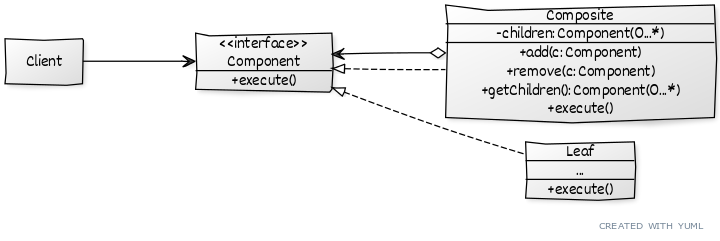
\includegraphics[width=0.8\linewidth]{images/CompositeUml}
	\caption{Diagram UML wzorca kompozyt.}
	\label{lab3/fig/CompositeUml}
\end{figure}
%[Client]->[Component]
%[Component]^-.-[Composite]
%[Composite]<>->[Component]
%[Component]^-.-[Leaf]
%
%[Client]
%[<<interface>>Component|+execute()]
%[Leaf|...|+execute()]
%[Composite|-children: Component(0...*)|+add(c: Component);+remove(c: Component);+getChildren(): Component(0...*);+execute()]

Jako przykład wykorzystania wzorca wyobraźmy sobie drzewo składające się z produktów oraz pudełek (kontenerów) które te produkty przechowują. Zarówno liście jak i kontenery implementują wspólny interfejs. Klient wywołuje metodę np. \texttt{GetPrice()} głównego kontenera (korzenia). Jeśli dzieckiem danego wierzchołka jest liść (produkt) zwracana jest jego cena, żądanie zostaje obsłużone bezpośrednio. Jeśli natomiast dzieckiem jest inny kontener (obiekt \texttt{Composite}), to przeglądana jest jego zawartość i ponownie w zależności od zawartości podejmowana jest akcja dotycząca dalszego przeglądania albo zwrócenia ceny.

Interfejsy graficzne, systemy SCADA zwykle pozwalają na rysowanie złożonych elementów z wielu innych, prostszych elementów. Klient nie chce traktować prostych i złożonych elementów w odmienny sposób. Powodowałoby to dodatkowe skomplikowanie modułu programu. Klasy \texttt{Line}, \texttt{Rectangle}, \texttt{Text} definiują proste elementy graficzne. Klasa \texttt{Picture} natomiast mogłaby stanowić kontener, w którym były przechowywane proste elementy podrzędne. Jest to jeden z przykładów, gdzie mógłby zostać wykorzystany wzorzec projektowy Kompozyt.

\subsubsection{Zadanie 2}

Jak w zadaniu pierwszym utwórz nowy projekt (aplikację konsolową .NET 5.0). Dodaj w nim folder o~nazwie \texttt{Equipments}. Wewnątrz tego folderu dodaj klasę abstrakcyjną komponentu \texttt{Equipment}\ref{lab3/lst/compositeAbstractClass}. Definiuje ona wspólny dla wszystkich klas interfejs. To po niej będą dziedziczyły klasy liści oraz kompozytów (kontenerów). Struktura drzewiasta będzie zawierała elementy komputera PC. Płyta główna i obudowa będą pełnić funkcję kontenerów natomiast procesor, pamięć RAM oraz dysk twardy będą pełnić funkcję liści.
\begin{lstlisting}[caption={Przykład abstrakcyjnej klasy komponentu}, label={lab3/lst/compositeAbstractClass}]
abstract class Equipment
{
	public abstract decimal NetPrice();
	public abstract decimal DiscountPrice();	
	public abstract int Power();
	public virtual void Add(Equipment component) => throw new NotImplementedException();	
	public virtual void Remove(Equipment component) => throw new NotImplementedException();
	public virtual bool IsComposite() => true;
}
\end{lstlisting}
%Normlanie lepiej byłoby zamiast stosować podstawowe typu utworzyć klasę Currency.
Następnie w tym samym projekcie dodaj klasy zarówno kontenerów np. \texttt{Chasis} oraz \texttt{Motherboard} oraz liści np. \texttt{Cpu}, \texttt{FloppyDisk}. Wszystkie powinny dziedziczyć po klasie \texttt{Equipment}. Przykładowa implementacja klasy \texttt{FloppyDisk} została pokazana na listingu~\ref{lab3/lst/compositeLeafFloppyDisk}.
\begin{lstlisting}[caption={Przykład klasy będącej liściem kompozytu}, label={lab3/lst/compositeLeafFloppyDisk}]
class FloppyDisk : Equipment
{
	private readonly decimal price;
	private readonly decimal discount;
	private readonly int power;
	
	public FloppyDisk(decimal price, decimal discount, int power)
	{
		this.price = price;
		this.discount = discount;
		this.power = power;
	}

	public override decimal NetPrice() => price;	
	public override bool IsComposite() => false;	
	public override decimal DiscountPrice() => price * (1 - discount);
	public override int Power() => power;
}
\end{lstlisting}
Klasa kontenera dodatkowo powinna posiadać pole listy na inne kontenery i liście oraz implementować metody wirtualne \texttt{Add} oraz \texttt{Remove}. Wspomniana lista może przechowywać zarówno obiekty kontenerów jak i~liści ponieważ oba typy dziedziczą po tej samej klasie abstrakcyjnej. Metody \texttt{NetPrice}, \texttt{DiscountPrice} oraz \texttt{Power} klasy kontenera powinny przeglądać dodane wcześniej komponenty (liście lub inne kontenery) i zwracać sumę cen wszystkich elementów podrzędnych. Fragment klasy \texttt{MotherBoardEquipment} wraz z~metodą zwracającą wartość będącą sumą cen wszystkich elementów pokazano na listingu~\ref{lab3/lst/compositeEquipmentClass}.
\begin{lstlisting}[caption={Fragment klasy \texttt{MotherBoardEquipment}}, label={lab3/lst/compositeEquipmentClass}]
class MotherBoardEquipment : Equipment
{
	protected List<Equipment> equipments = new List<Equipment>();

	//...
		
	public override void Add(Equipment component) => equipments.Add(component);	
	public override void Remove(Equipment component) => equipments.Remove(component);
	public override decimal NetPrice()
	{
		decimal result = price;
		equipments.ForEach(x => result += x.NetPrice());	
		return result;
	}
		
	//...
}
\end{lstlisting}

W klasie klienta, albo w metodzie \texttt{Main} sprawdź poprawność stworzonej struktury. Utwórz obiekt obudowy (\texttt{ChasisEquipment}) oraz dodaj do niego (za pomocą metody \texttt{Add}) kilka dysków twardych \texttt{FloppyDisk} oraz płytę główną \texttt{MotherBoardEquipment} do której wcześniej dodaj procesor \texttt{Cpu}.

Tak utworzoną strukturę przekaż do innej klasy klienckiej. Zwróć uwagę, że z punktu widzenia klienta nie ma znaczenia czy korzysta on z pojedynczego elementu liścia (np. klasy reprezentującej procesor) czy z~kontenera, który zawiera wiele dodatkowych elementów podrzędnych. Złożoność struktury drzewiastej jest przed nim ukryta przy pomocy wzorca Kompozyt.
\begin{lstlisting}
class Client
{
	public void PrintBill(Equipment equipment)
	{
		Console.WriteLine($"Bill:\n\t{equipment.NetPrice()}\n\t{equipment.DiscountPrice()}\n\t{equipment.Power()}");
	}
}
\end{lstlisting}

\subsection{Fasada (ang. facade)}
Jeśli istnieje potrzeba, aby ukryć złożoność całej biblioteki albo pewnego zbioru wielu klas można użyć wzorca projektowego Fasada (diagram UML przedstawiono na rysunku~\ref{lab3/fig/FacadeUml}). Jest to wzorzec upraszczający sposób w jaki klienci korzystają z współpracujących, zależnych od siebie klas. Fasada udostępnia jednolity interfejs dla zbioru interfejsów z podsystemu. Wykorzystując Fasadę klient nie musi tworzyć, ani zarządzać zależnościami pomiędzy obiektami, są one przed nim ukryte za interfejsem Fasady. Wzorzec ten może również służyć za punkt wejścia dla podsystemu w~warstwowo podzielonym zestawie.

Fasada pozwala zmniejszyć liczbę obiektów z której korzystają klienci. Dodatkowo wprowadza luźne powiązanie pomiędzy klientami, a podsystemami. Ułatwione jest dzięki temu wprowadzanie zmian w~podsystemach jak również zmiana zależności między nimi. 

\begin{figure}[hbt!]
	\centering
	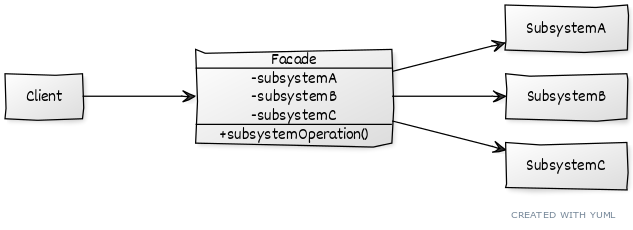
\includegraphics[width=0.8\linewidth]{images/FacadeUml}
	\caption{Diagram UML wzorca Fasada.}
	\label{lab3/fig/FacadeUml}
\end{figure}
%[Client]->[Facade]
%[Facade]->[SubsystemA]
%[Facade]->[SubsystemB]
%[Facade]->[SubsystemC]
%
%[Client]
%[Facade|-subsystemA;-subsystemB;-subsystemC|+subsystemOperation()]
%[SubsystemA]
%[SubsystemB]
%[SubsystemC]

Interfejs udostępniany przez omawiany wzorzec jest uproszczony. Klasa Fasady nie musi korzystać z~wszystkich funkcjonalności klas, które wykorzystuje. Dostarczane są jedynie te niezbędne. 
%Jedynie bardziej wymagający klienci będą musieli spojrzeć za fasadę.

Przykładem zastosowania Fasady może być ukrycie złożoności procesu konwersji materiału wideo. Klient \textbf{nie} korzystający z omawianego wzorca byłby zmuszony do wykorzystywania różnych klas. Inna klasa zostałaby użyta do kompresji materiału wideo inna do miksowania audio, a jeszcze inna do zmiany formatu pliku. Klient może potrzebować jedynie uproszczonego interfejsu do konwertowania pliku wideo. Nie interesują go złożone mechanizmy tego procesu. Dlatego zamiast zmuszać klienta do posiadania i zarządzania wieloma klasami, można utworzyć klasę fasady, która te złożoności przed nim ukryje. Jeśli w przyszłości część wykorzystywanych klas się zmieni, aktualizacja kodu będzie wymagana tylko w klasie Fasady.

Innym przykładem, gdzie omawiany wzorzec ma zastosowanie jest podsystem kompilujący. Również w~tym przypadku klienta nie interesują złożone zależności pomiędzy parserem, preprocesorem, analizatorem semantyki czy optymalizatorem. Autorzy klientów chcą tylko skompilować kod. Jeśli proces kompilacji zostanie ukryty w~pojedynczej klasie \texttt{Compiler}, to będzie ona odgrywała rolę fasady.
% g++ -Wall -std=c++14 main.cpp -o main.exe //-Wall (all warnings) and -o main.exe instead of a.exe

\subsubsection{Zadanie 3}

Utwórz kolejny projekt w~analogiczny jak w poprzednich zadaniach sposób. Tym razem zostanie wykorzystany wzorzec projektowy Fasady do ukrycia złożoności serwisów odpowiedzialnych za pobieranie informacji o ,,danych meteorologicznych''.

Dodaj do projektu folder \texttt{WeatherServices}. Następnie umieść w nim trzy interfejsy w osobnych plikach: \texttt{ITemperatureService}, \texttt{IHumidityService} oraz \texttt{IForecastService}. Każdy z nich niech deklaruje jedną metodę: \texttt{double GetTemperature()}, \texttt{double GetHumidity()} i \texttt{double GetForecast()}. 

Dodaj do tego samego folderu trzy klasy implementujące te interfejsy. W celu wygenerowania pomiarów możesz skorzystać z~generatora liczb pseudolosowych np. klasy \texttt{System.Random} i jej metody \texttt{NextDouble}. Generacja liczb z pewnego przedziału może być zrealizowana w następujący sposób:
\begin{lstlisting}	
random.NextDouble() * (maxValue - minValue) + minValue;
\end{lstlisting}
%To generate a cryptographically secure random number, such as one that's suitable for creating a random password, use the RNGCryptoServiceProvider class or derive a class from System.Security.Cryptography.RandomNumberGenerator.
Można również wykorzystać Metodę Rozszerzającą (ang. Extension Method)\footnote{Metody rozszerzające pozwalają na ,,dodanie'' metody do już istniejącego typu, bez konieczności tworzenia nowej klasy pochodnej czy modyfikacji klasy już istniejącej. Metody rozszerzające są statyczne, ale ich wywołanie wygląda jakby należało do instancji danej klasy. Kompilator tłumaczy wywołanie tej metody na metodę statyczną. 
% Enkapsulacja nie jest naruszona, metody rozszerzajace nie maja dostepu do składowych prywatnych.
}. Dodaj do projektu folder \texttt{Extensions}, a w nim statyczną klasę \texttt{RandomExtension}. W  klasie natomiast dodaj statyczną metodę \texttt{NextDouble} o następującej postaci:
\begin{lstlisting}	
public static class RandomExtensions
{
	public static double NextDouble(this Random random, double minValue, double maxValue)
	{
		return random.NextDouble() * (maxValue - minValue) + minValue;
	}
}
\end{lstlisting}
Zwróć uwagę na pierwszy parametr, określa on do jakiego typu (klasy) chcemy ,,dodać'' nową metodę. Konieczne jest, aby poprzedzić go słowem kluczowym \texttt{this}. Kolejne parametry nie różnią się niczym od tych ze standardowej deklaracji metody.

Po dodaniu klasy \texttt{RandomExtension} klasa \texttt{Random} ,,otrzymała'' nową metodę, która generuje liczbę pseudolosową typu \texttt{double} z określonego przez klienta przedziału. Metod rozszerzających nie należy stosować tam gdzie możemy modyfikować kod klasy, dodać składową. Jest to jednak dobre narzędzie jeśli chcemy dodać funkcjonalność do kodu, który nie jest pod naszą kontrolą, a dziedziczenie jest nieodpowiednie albo niemożliwe. 

Klasy implementujące utworzone wcześniej interfejsy mogą teraz wykorzystywać metody rozszerzające. Listing~\ref{lab3/lst/temperatureServiceExtensionMethod} przedstawia przykładową implementację klasy \texttt{TemperatureService}.
\begin{lstlisting}[caption={Fragment klasy \texttt{TemperatureService} wykorzystującej metodę rozszerzającą}, label={lab3/lst/temperatureServiceExtensionMethod}]	
public class TemperatureService : ITemperatureService
{
	public double GetTemperature() => new Random().NextDouble(-20, 40);
}
\end{lstlisting}

Dalej dodaj do głównego katalogu projektu plik z rekordem\footnote{Słowo kluczowe \texttt{record} wraz z \texttt{init} pojawiło się C\# 9.0 i pozwala zdefiniować typ referencyjny, który służy do przechowywania danych. Tworzone w ten sposób typ jest \textbf{niezmienny} tzn. stan takiego obiektu nie może się zmienić po jego utworzeniu. Zmiana jego stanu jest możliwa jedynie poprzez utworzenie nowej instancji. Rekordy pozwalają na utworzenie nowego obiektu bez konieczności przepisywania wszystkich właściwości, jedna po drugiej. Można posłużyć się słowem kluczowym \texttt{with} i zmienić jedną właściwość, pozostałe zostaną natomiast przepisane automatycznie. Przed pojawieniem się rekordów konieczne było tworzenie właściwości jedynie z akcesorem \texttt{get} oraz ustawianie ich w konstruktorze za pomocą przekazanych przez klienta argumentów.} \texttt{Weather}:
\begin{lstlisting}	
public record Weather(double Temperature, double Humidity, double Forecast);
\end{lstlisting}

Umieść z katalogu głównym nową klasę Fasady dla wcześniej stworzonych serwisów. Klasa Fasady niech zawiera trzy pola w których przechowasz referencję do obiektów implementujących utworzone wcześniej interfejsy. W konstruktorze przypisz im przekazane przez parametry konstruktora obiekty. Dodaj również metodę \texttt{GetWeatherInformation} zwracającą obiekt typu \texttt{Weather}. Metoda ta niech pobiera informacje o~temperaturze, wilgotności oraz estymacji przekazanych serwisów i zwraca jeden obiekt zawierający te dane:
\begin{lstlisting}	
public class WeatherApiFasade
{
	//...
	
	public WeatherApiFasade(ITemperatureService temperatureService, 
		IHumidityService humidityService, IForecastService forecastService)
	{
		//...
	}
	
	public Weather GetWeatherInformation()
	{
		return  new(
			temperatureService.GetTemperature(),
			humidityService.GetHumidity(),
			forecastService.GetForecast());
	}
}
\end{lstlisting}

Na koniec dodaj do projektu klasę \texttt{Application}:
\begin{lstlisting}	
class Application
{
	public static void Run(WeatherApiFasade weatherApiFasade)
	{
		Console.Write(weatherApiFasade.GetWeatherInformation());
	}
}
\end{lstlisting}
W metodzie \texttt{Main} utwórz obiekt typu \texttt{WeatherApiFasade} przekazując do niego wcześniej utworzone obiekty wymagane przez konstruktor. Wywołaj metodę \texttt{Run()} i sprawdź czy na ekranie konsoli zostały wypisane oczekiwane wyniki:
\begin{lstlisting}	
static void Main(string[] args)
{
	WeatherApiFasade weatherApiFasade = new WeatherApiFasade(
		new TemperatureService(), 
		new HumidityService(),
		new ForecastService());
	
	Application.Run(weatherApiFasade);
}
\end{lstlisting}

%\clearpage
%\section{Wzroce projektowe (3) - czynnościowe }
\subsection{Polecenie (ang. command)}
Polecenie umożliwia zamianę żądania w samodzielny, osobny obiekt. Z tym wzorcem można się spotkać w~kontekście interfejsów użytkownika. Do przycisku może być przypisana akcja (obiekt implementujący interfejs \texttt{ICommand}). Obiekt przycisku powinien posiadać pole/właściwość typu \texttt{ICommand}, można ją przekazać np. jako argument konstruktora. Po kliknięciu w element, instancja przycisku nie jest świadoma akcji, która powinna się wykonać. Pozwala to na łatwą zmianę działania przycisku i umożliwia zachowanie zasady pojedynczej odpowiedzialności (komponent odpowiedzialny za interfejs graficzny nie jest świadomy działania pozostałych warstw aplikacji). Chcąc wprowadzić nową funkcjonalność wystarczy stworzyć nowy obiekt implementujący \texttt{ICommand} i przekazać go do nadawcy (utrzymana jest tym samym zasada otwarte/zamknięte). 

Co więcej, wykorzystanie wzorca Polecenie pozwala na przypisanie kilku przyciskom tej samej czynności. Na przykład operacja zapisywania może być dostępna zarówno jako osobny przycisk jak i~kombinacja klawiszy \texttt{Ctrl+S}.

Dodatkowo omawiany wzorzec pozwala na implementacje cofania, ponawiania operacji oraz ich kolejkowania. Możliwe jest również łączenie wielu prostych poleceń w jedno bardziej skomplikowane.

Jeśli obiekt polecenia do wykonania żądania wymaga dodatkowych parametrów (np. z pól formularza), należy je przekazać jako argument konstruktora (jeśli obiekt ma być niezmienny) albo przez jego właściwości.


%Innym podejściem mogłoby być stworzenie wielu klas dziedziczących po klasie Button np. OkButton, CancelButton, ApplyButton itp...

%Warto zwrócić uwagę na wzorzec MVVM i jak Microsoft podszedł do tematu obłsugi przycisków UI


%PRZYKŁAD Z REFACTORING GURU: Podczas długiego spaceru po mieście, docierasz do miłej restauracji i siadasz przy oknie. Przyjazny kelner szybko przyjmuje zamówienie, spisując je na małym kawałku papieru. Następnie kelner idzie do kuchni i przykleja kartkę na ścianie. Po jakimś czasie zamówienie dociera do szefa kuchni, który przygotowuje danie, a następnie umieszcza posiłek na tacce wraz z zamówieniem. Kelner znajduje tackę, sprawdza zgodność z zamówieniem i zanosi ją do stolika. Zamówienie na papierze stanowi polecenie. Trafia do kolejki, do momentu aż szef kuchni je przygotuje. Zamówienie zawiera wszystkie niezbędne informacje wymagane do przygotowania posiłku. Umożliwia to kucharzowi rozpoczęcie gotowania od razu, zamiast ustalać szczegóły z klientem na własną rękę.


\begin{figure}[hbt!]
	\centering
	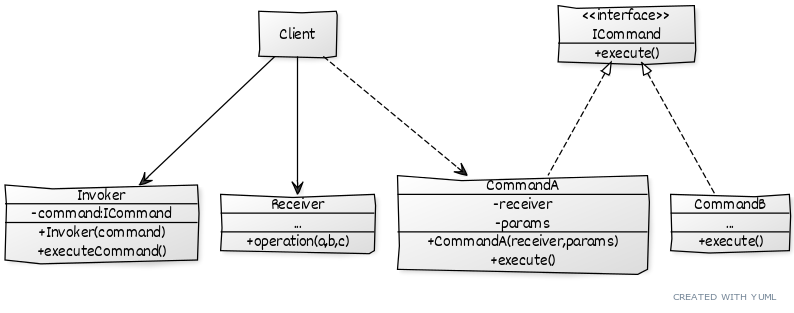
\includegraphics[width=0.9\linewidth]{images/CommandUml}
	\caption{Diagram UML wzorca Polecenie.}
	\label{lab4/fig/CommandUml}
\end{figure}
%[Client]->[Invoker]
%[Client]->[Receiver]
%[Client]-.->[CommandA]
%[ICommand]^-.-[CommandA]
%[ICommand]^-.-[CommandB]
%
%[Client]
%[Invoker|-command:ICommand|+Invoker(command);+executeCommand()]
%[≪interface≫;ICommand|+execute();]
%[CommandA|-receiver;-params|+CommandA(receiver,params);+execute()]
%[CommandB|...|+execute()]
%[Receiver|...|+operation(a,b,c)]

\subsubsection{Zadanie 1}
Utwórz projekt aplikacji konsolowej .NET 5.0. W nowym pliku dodaj interfejs \texttt{ICommand} z dwiema deklaracjami metod: \texttt{void Execute()} oraz \texttt{void Undo()}.

Dodaj klasę \texttt{Character} z jedną publiczną właściwością typu \texttt{Vector3} o nazwie \texttt{Position} (konieczne będzie dodanie przestrzeni nazw \texttt{using System.Numerics}):
\begin{lstlisting}
public class Character
{
	public Vector3 Position { get; set; }
}
\end{lstlisting}

Następnie do projektu dodaj klasę o nazwie \texttt{Move} implementującą interfejs \texttt{ICommand}. Niech posiada ona konstruktor z trzema parametrami, określającymi obiekt do przesunięcia, wektor o jaki ma zostać przesunięty obiekt oraz długość przesunięcia (domyślnie równą jeden):
\begin{lstlisting}
public class Move : ICommand
{
	private readonly Character objectToMove;
	private readonly Vector3 direction;
	private readonly float distance;
	
	public Move(Character objectToMove, Vector3 direction, float distance = 1f)
	{
		this.objectToMove = objectToMove;
		this.direction = direction;
		this.distance = distance;
	}

	//...
\end{lstlisting}
Aby skorzystać ze struktury \texttt{Vector3} również konieczne jest dodanie przestrzeni nazw \texttt{System.Numerics} w~tej klasie. Zaimplementuj w~\texttt{Move} interfejs, tak aby po wywołaniu metody \texttt{Execute()} pozycja przekazanego w konstruktorze obiektu została zaktualizowana o wektor \texttt{direction} (również przekazany jako argument konstruktora) np. w następujący sposób:
\begin{lstlisting}
public class Move : ICommand
{
	//...	
	public void Execute() => objectToMove.Position += direction * distance;
	//...
}
\end{lstlisting}
Analogicznie zaimplementuj operację \texttt{Undo()}.

Wzorzec Polecenie często jest wykorzystywany do przechowywania, cofania i ponawiania jakieś operacji. Dodaj do projektu klasę \texttt{CommandHandler}, która będzie odpowiedzialna za przechowywanie poleceń i~umożliwiała ich cofanie oraz ponowne wywoływanie:
\begin{lstlisting}
public class CommandHandler
{
	private readonly Stack<ICommand> commands = new();
	private readonly Stack<ICommand> redos = new();
	
	public void Add(ICommand command){}
	public void Undo(){}
	public void Redo(){}
}
\end{lstlisting}
Zaimplementuj metody: \texttt{Add}, \texttt{Undo} oraz \texttt{Redo}.

Następnie w klasie \texttt{Character} dodaj prywatne pole typu \texttt{CommandHandler}. Dodatkowo umieść w~niej metody \texttt{Move}, \texttt{Undo} oraz \texttt{Redo}. Będą one obsługiwać operacje ,,przesuwania'' obiektu typu \texttt{Character} wykorzystując \texttt{CommandHandler}.
\begin{lstlisting}
public class Character
{
	public Vector3 Position { get; set; }
	private readonly CommandHandler commands = new();
	
	public void Move(ICommand command)
	{
		commands.Add(command);
		this.PrintPosition();
	}
	
	public void Undo()
	{
		//...
	}
	
	public void Redo()
	{
		//...
	}
	
	private void PrintPosition() => Console.WriteLine(\$"Current position: {this.Position}");
}
\end{lstlisting}
Dodaj implementację metod \texttt{Undo} oraz \texttt{Redo}.

W metodzie \texttt{Main} dodaj obiekt typu \texttt{Character} i cztery obiekty typu \texttt{Move}, następnie wywołując metody \texttt{Move}, \texttt{Undo} i \texttt{Redo} zbadaj poprawność napisanych klas:
\begin{lstlisting}
class Program
{
	static void Main(string[] args)
	{
		var character = new Character();
		ICommand left = new Move(character, new Vector3(-1f,0f,0f), 1f);
		ICommand right = new Move(character, new Vector3(1f, 0f, 0f), 1f);
		ICommand up = new Move(character, new Vector3(0f, 1f, 0f), 1f);
		ICommand down = new Move(character, new Vector3(0f, -1f, 0f), 1f);
		
		character.Move(left);
		character.Move(up);
		character.Move(up);
		character.Undo();
		character.Redo();
	}
}
\end{lstlisting}

\subsection{Strategia (ang. strategy)}\label{lab4/sec/strategy}

Klient, aby zrealizować pewne zadania może wykorzystywać konkretny algorytm. Często może się on zmieniać w~czasie albo być zależny od dodatkowych czynników np. wyboru opcji przez użytkownika programu. Wzorzec Strategia pozwala utworzyć rodzinę algorytmów realizujących dane zadanie w różny sposób. Dalej za pomocą konstruktora, właściwości albo metody klient może podmienić obiekt strategii i tym samym zmienić sposób realizacji danej czynności przez daną klasę. Gorszą alternatywą mogłoby być zbudowanie na stałe wielu algorytmów w daną klasę i naruszenie tym samym pierwszych dwóch zasad \textbf{SO}LID (\ref{lab1/sec/srpPrinciple} i \ref{lab1/sec/ocpPrinciple}).

Strategia bazuje na mechanizmie odwracania zależności. Koncepcyjnie DI jest raczej zarezerwowane dla przypadków, gdzie podczas wykonywania się programu dane zachowanie (wstrzykiwany obiekt) jest stałe. Jeśli natomiast zakładamy, że sposób realizacji danego algorytmu będzie się zmieniał to wtedy odnosimy się raczej do wzorca Strategia. Różnice między nimi są niewielkie i subtelne. Pod względem struktury strategia jest podobna również do mostu i stanu, które też bazują na kompozycji. Mimo, że pod względem struktury są ona do siebie bardzo podobne, nazewnictwo stosowane w tych wzorcach powinno programistę informować o~specyficznym problemie, który został za jego pomocą rozwiązany.

W programowaniu obiektowym istnieje zasada, aby przekładać kompozycję nad dziedziczeniem. Podobnym do strategii wzorcem jest również Metoda Szablonowa wykorzystująca dziedziczenie. Takie podejście sprawia, że strategia jest na sztywno połączona z~klasa \texttt{Context}, nie możliwe jest dynamiczne zmienianie algorytmu. Dodatkowo utrudnia to zrozumienie kodu. 

%Refactoring guru
%Polecenie i Strategia mogą wydawać się podobne, ponieważ oba mogą służyć parametryzacji obiektu jakimś działaniem. Mają jednak inne cele. Za pomocą Polecenia można konwertować dowolne działanie na obiekt. Parametry działania stają się polami tego obiektu. Konwersja zaś pozwala odroczyć wykonanie działania, kolejkować je i przechowywać historię wykonanych działań, a także wysyłać polecenia zdalnym usługom, itd. Z drugiej strony, Strategia zazwyczaj opisuje różne sposoby wykonywania danej czynności, pozwalając zamieniać algorytmy w ramach jednej klasy kontekstu.

Diagram UML omawianego wzorca został przedstawiony na diagramie UML~\ref{lab4/fig/StrategyUml}. Klient tworzy obiekt konkretnej strategi (musi ona implementować wspólny dla wszystkich strategi interfejs). Dalej taka instancja może zostać przekazana np. przy wykorzystaniu metody (\texttt{setStrategy(strategy)}) do obiektu realizującego daną czynność. Klient ma możliwość w trakcie działania programu płynnie zmieniać sposób realizowania danej czynności.

\begin{figure}[hbt!]
	\centering
	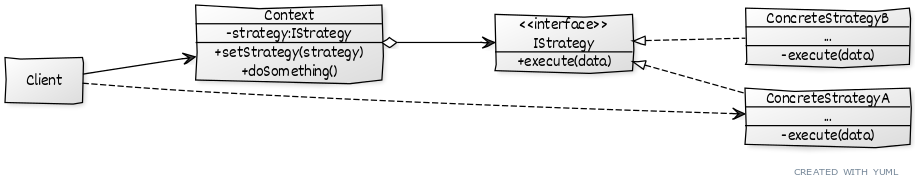
\includegraphics[width=0.9\linewidth]{images/StrategyUml}
	\caption{Diagram UML wzorca Strategia.}
	\label{lab4/fig/StrategyUml}
\end{figure}
%[Client]->[Context]
%[Client]-.->[ConcreteStrategyA]
%[Context]<>->[IStrategy]
%[IStrategy]^-.-[ConcreteStrategyA]
%[IStrategy]^-.-[ConcreteStrategyB]
%
%[Client]
%[Context|-strategy:IStrategy|+setStrategy(strategy);+doSomething()]
%[≪interface≫;IStrategy|+execute(data);]
%[ConcreteStrategyA|...|-execute(data)]
%[ConcreteStrategyB|...|-execute(data)]

%Użycie wzorca strategii powinno być podyktowane faktem, że klasa korzysta z różnych algorytmów do wykonania \textbf{tej samej} czynności. Co więcej, zwykle te algorytmy mogą się zmieniać w czasie. Dodatkowo algorytm ułatwia odizolowanie algorytmu od logiki biznesowej. Pozwala również ukryć szczegóły implementacyjne np. złożone struktury danych. 

Jeżeli obiekt strategi potrzebuje dodatkowych argumentów mogą one zostać udostępnione przez kontekst w~momencie wywoływania algorytmu. Ewentualnie \texttt{Context} może przekazać do obiektu strategii samego siebie.

Przykładem zastosowania wzorca Strategia może być nawigacja i różne algorytmy obliczania optymalnej drogi. Na przykład w~zależności od środka transportu może być stosowany inny obiekt \texttt{ConcreteStrategy}. W~bibliotece \texttt{ObjectWindows} strategia jest stosowana w oknach dialogowych do sprawdzania poprawności wprowadzanych przez użytkownika danych. Zestaw oferuje część predefiniowanych algorytmów, a~użytkownik jeśli nie znajdzie dla niego odpowiedniego, może łatwo rozszerzyć możliwości przez stworzenie własnego obiektu implementującego konkretny interfejs. Strategia może również być wykorzystywana w~algorytmach parsujących (różne algorytmy w zależności od formatu danych wejściowych) albo optymalizacji kompilowanego kodu (inne obiekty dla poszczególnych rodzajów i poziomów kompilacji).

\subsubsection{Zadanie 2}
W solucji dodaj kolejny projekt aplikacji konsolowej .NET 5.0. Dodaj w nim interfejs \texttt{IRouteStrategy} z~jedną metodą \texttt{BuildRoute}, nie przyjmującą żadnych argumentów i~zwracającą typ \texttt{void}. 

Następnie dodaj trzy klasy: \texttt{PublicTransportStrategy}, \texttt{RoadStrategy} i \texttt{WalkingStrategy} implementujące interfejs \texttt{IRouteStrategy} np. w następujący sposób:
\begin{lstlisting}
public class PublicTransportStrategy : IRouteStrategy
{
	public void BuildRoute() => Console.WriteLine("Public transport strategy has been used for travel time estimation.");
}
\end{lstlisting}

Dalej dodaj do projektu klasę \texttt{Navigator} z konstruktorem przyjmującym argument typu \texttt{IRouteStrategy} i przypisującym go do prywatnego pola. 

Dodatkowo w klasie \texttt{Navigator} dodaj dwie metody: \texttt{SetStrategy} oraz \texttt{Navigate}:
\begin{lstlisting}
public class Navigator
{
	//...
	
	public void SetStrategy(IRouteStrategy strategy) => this.routeStrategy = strategy;
	
	public void Navigate() => this.routeStrategy.BuildRoute(); //in real scenario method should return direction, trace from point A to point B
}
\end{lstlisting}

W metodzie \texttt{Main} sprawdź działanie przykładowego programu:
\begin{lstlisting}
static void Main(string[] args)
{
	var context = new Navigator(new RoadStrategy());
	context.Navigate();
	
	context.SetStrategy(new PublicTransportStrategy());
	context.Navigate();
	
	context.SetStrategy(new WalkingStrategy());
	context.Navigate();
}
\end{lstlisting}

Oczywiście metody \texttt{BuildRoute} w~normalnym przypadku powinny przyjmować współrzędne lokalizacyjne i~zwracać faktyczną drogę umożliwiającą przemieszczenie się z~punktu A do punktu B.

\subsection{Mediator (ang. mediator)}

Wzorzec projektowy mediator umożliwia kapsułkowanie interakcji pomiędzy obiektami poprzez dodatkowy obiekt mediatora. Obiekty mogą się komunikować jedynie wykorzystując ten obiekt.

%Analogią może być wieża kontrolerów lotów na lostniku. Piloci nie rozmawiają między sobą nawzajem, a komunikują się przez swego rodzaju moderatora. 

Wyobraźmy sobie sytuację, w której okno dialogowe składa się z wielu widgetów. Pewne pole może być aktywne albo nieaktywne w zależności od wybranej wcześniej opcji widgetu typu \texttt{checkbox}. W innym przypadku przycisk do wysłania formularza aktywowany jest dopiero po wypełnieniu wszystkich niezbędnych pól. Bez użycia obiektu mediatora poszczególne instancje widgetów musiałby posiadać referencje do sobie nawzajem, aby np. po zaznaczeniu pola wyboru, aktywować pole tekstowe. Ponowne użycie takich elementów staje się utrudnione, a czytelność kodu się pogarsza.


Zamiast zmuszać obiekty do posiadania informacji o sobie nawzajem można wprowadzić dodatkowy obiekt moderatora (diagram UML przedstawiono poniżej\ref{lab4/fig/MediatorUml}), który będzie pośredniczył w~komunikacji między obiektami. Komponenty w tej sytuacji są zależne jedynie od obiektu moderatora i to do niego kierują informację np. o zmianie stanu pola wyboru. Na przykład momencie kliknięcia przycisku przez użytkownika obiekt \texttt{Button} mógłby wysyłać informację o~operacji do mediatora, który sprawdzałby pozostałe pola i podejmował decyzję o wysłaniu formularza. 


Obiekty mogą się komunikować np. z~wykorzystaniem zdarzeń albo wzorca obserwatora. We wzorcu MVC (ang. Model View Controller - Model Widok Kontroler) moderatorem jest kontroler.

\begin{figure}[hbt!]
	\centering
	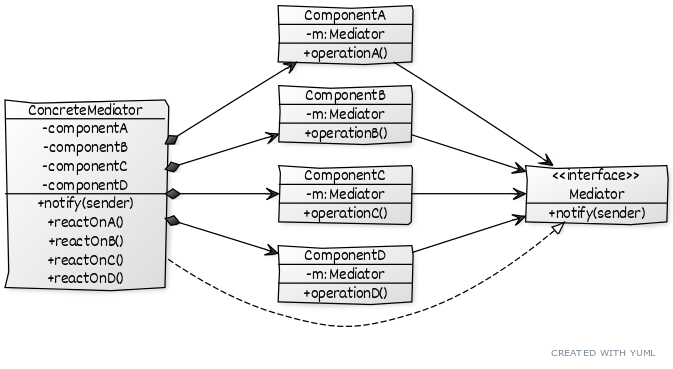
\includegraphics[width=0.9\linewidth]{images/MediatorUml}
	\caption{Diagram UML wzorca Mediator.}
	\label{lab4/fig/MediatorUml}
\end{figure}
%[ConcreteMediator]++->[ComponentA]
%[ConcreteMediator]++->[ComponentB]
%[ConcreteMediator]++->[ComponentC]
%[ConcreteMediator]++->[ComponentD]
%[Mediator]^-.-[ConcreteMediator]
%[ComponentA]->[Mediator]
%[ComponentB]->[Mediator]
%[ComponentC]->[Mediator]
%[ComponentD]->[Mediator]
%
%[≪interface≫;Mediator|+notify(sender)]
%[ConcreteMediator|-componentA;-componentB;-componentC;-componentD|+notify(sender);+reactOnA();+reactOnB();+reactOnC();+reactOnD()]
%[ComponentA|-m: Mediator|+operationA()]
%[ComponentB|-m: Mediator|+operationB()]
%[ComponentC|-m: Mediator|+operationC()]
%[ComponentD|-m: Mediator|+operationD()]

Wzorzec Mediator warto zastosować jeśli istnieje wiele zależności pomiędzy klasami, a ich ponowne użycie w~innym programie jest z tego powodu mocno utrudnione. Podobnym wzorcem do Mediatora jest Fasada. Główną różnicą między nimi jest fakt, że ta druga posiada zależności jednokierunkowe. Obiekty reprezentowane przez fasadę mogą kierować żądania do podsystemów, ale podsystemy nie mogą komunikować się z Fasadą.

Wadą omawianego wzorca jest fakt, że mediator z czasem może stać się bardzo złożony tzw. Boski Obiekt. Taki obiekt jest przykładem antywzorca projektowego. Posiada on zazwyczaj wiele zależności i~łamie zasadę pojedynczej odpowiedzialności. Dodatkowo należy szczególnie zaznaczyć, że Mediator powinien być używany w~większych projektach. Wprowadza on dodatkową złożoność. Tak samo jak z większością wzorców projektowych jeśli tworzymy proste aplikacje, albo krótkie przykłady tak jak na laboratoriach to użycie niektórych wzorców jest niepożądane. Nie ma sensu komplikować prostego, małego projektu.
Jeśli jednak aplikacja zaczyna się rozrastać to dobre praktyki i wzorce zaczynają mieć znaczenie. %Trochę jak z huśtawką rozmiar i złożoność aplikacji musimy równoważyć dobrymi wzorcami i zasadami czy liczbą testów. 
Tak samo Madiator jak i opisany w~kolejnych akapitach wzorzec CQRS \textbf{nie są} korzystne dla wszystkich aplikacji.

%\subsubsection{Jason Taylor - CleanArchitecture}
%Solucja powinna być podzielona na odpowiednie komponenty. Nie ma sensu tworzyć ogromnej ilości osobnych zestawów, które mogłyby zostać umieszczone w folderach. Należy natomiast w przemyślany sposób komponenty rozdzielać od siebie tam gdzie jest to przydatne. 
%
%W pierwszej kolejności warto oddzielić kod źródłowy oprogramowania od testów. Można to zrealizować przez stworzenie dwóch osobnych folderów. W pierwszym można umieścić cztery warstwy np.:
%\begin{itemize}
%	\item Application - zawiera logikę związaną w aplikacją. Związana jest z warstwą domeny i niczym więcej. Definiuje ona interfejsy, które powinny być implementowane na przez zewnętrzne warstwy t.j. infrastrukturę oraz WebUI. Jeśli aplikacja wymaga dostępu do serwisu powiadomień, interfejs powinien znaleźć się w warstwie aplikacji, natomiast jego implementacja w infrastrukturze.
%	\item Domain - przechowuje encję, typy wyliczeniowe, wyjątki, interfejsy, typy i logikę specyficzną dla warstwy domeny. Jeśli piszemy projekt związany z finansami to wszystko co ma związek z tą domeną powinno się tam znaleźć. Nie posiada żadnych dodatkowych zależności.
%	\item Infrastructure - zawiera klasy, które pozwalają na dostęp do zewnętrznych zasobów takich jak systemy plików, web serwisy, bazy danych itp. Powinny opierać się na interfejsach zdefiniowanych w warstwie aplikacji.
%	\item WebUI - warstwa prezentacji, odpowiada za interakcję z aplikację. Może to być aplikacja Anuglar, standardowy MVC, Blazor, WPF itp. Opiera się zarówno na warstwie aplikacji oraz infrastruktury. Przy czym należy mieć na uwadze, że powiązanie z warstwą infrastruktury istnieje jedynie, aby umożliwić wstrzykiwanie zależności. Jedynie \texttt{Startup.cs} powinien posiadać referencję do warstwy infrastruktury, w celu rejestracji serwisów.
%\end{itemize}
% Mamy cztery projekty i reprezentują one trzy warstwy. Od środką jest do po kolei domena, infrastruktura, aplikacja oraz WebUI. 
% WebUI jest warstwą prezentacji (najwyższą warstwą), odpowiada za interakcję z aplikacją. Może to być aplikacja Angular, MVC, Blazor, WPF itd.  
% Domain (Entities) np. ToDoItem oraz ToDoList plus osoby folder Exception, Enums, ValueObjects itd. Serce całej aplikacji.
% Application - odpwiada za to jak wykorzystywać encję z domeny. Np. posiada Commands typu. CreateToDoItem, CreateToDoList. Nie zawiera informacji JAK tworzyć te listy, gdzie je przechowywać itd.
% Infrastrature - implementuje abstrakcję z Application.
% WebUI - zależność od warstwy infrastruktury jedynie w celach rejestracji usług.
% Powyższe pozwala nam na czystą i prostą architekturę. 
% W osobnych folderze obok kodu źródłowego należy dodać testy jednostkowe. Osobno można dodać testy akceptacyjne, w innym projekcie związne w warstwą aplikacji i jeszcze w innym te związane z warstwą domeny.
% Jeśli WebUI jest API można go opublikować jako pakiet NuGet, aby innym koledzy z zespołu mogli z niego korzystać. 

\subsubsection{CQRS and MediatR framework}\label{sec/lab4/cqrs}

% Source : https://docs.microsoft.com/en-us/azure/architecture/patterns/cqrs

W prostych aplikacjach webowych często korzysta się z tzw. podejścia CRUD\footnote{Skrót CRUD (ang. Create Read Update Delete) określa cztery podstawowe operacje służące do utrwalania danych np. w bazie danych. Za pomocą tych operacji  np. interfejs użytkownika może dodawać, odczytywać, aktualizować i usuwać rekordy w~bazie danych.}. W sytuacji wielu zapytań o różne obiekty danych (DTO) aplikacja musi wykonywać wiele operacji mapowania. Dodatkowo proces zapisu może wymagać złożonej walidacji i dodatkowej logiki biznesowej. Powoduje to, że model staje się skomplikowany i trudny w utrzymaniu. Mimo tych wad CRUD jest bardzo często (i słusznie) stosowany w prostych aplikacjach. Jeśli domena jest prosta, albo CRUD jest wystarczający nie ma większego sensu stosować omówionego poniżej CQRS.
 
Wraz ze wzrostem złożoności aplikacji mogą pojawiać się dodatkowe problemy. Może okazać się konieczne łączenie wielu rekordów w jeden, albo łączenie kilku rekordów w~jeden wirtualny. W przypadku aktualizacji danych konieczna może być bardziej złożona walidacja danych. 
 
Pewnym rozwiązaniem ułatwiającym skalowanie oraz zapewnienie wysokiej wydajności jest wykorzystanie wzorca CQRS (ang. Command Quary Responsibility Segregation), który oddziela zapytania (Query) i polecenia (Command) do bazy danych. Zapytania \texttt{Queries} nie powinny modyfikować danych, mogą one jedynie czytać dane. Polecenia natomiast służą do dodawania nowych danych, usuwania ich albo aktualizacji. Używany jest inny model do zapisu i odczytu. Pisząc o różnych modelach mamy na myśli różne modele obiektów często działające w różnych procesach, albo na różnych maszynach. Np. w przypadku stron www renderowanie wykorzystuje model zapytań. Jeśli natomiast użytkownik wykona jakąś akcję np. danie kciuka w górę na portalu społecznościowym to takie polecenie jest wysyłane do osobnego modelu do przetworzenia. Innymi korzyściami jest zwiększenie bezpieczeństwa ponieważ ta sama encja nie jest wykorzystywana zarówno do operacji czytania i zapisywania. W przeciwnym przypadku informacje mogłyby zostać użyte w złym kontekście. 

Wykorzystywane modele są elastyczne i łatwe w~utrzymaniu. Skomplikowana logika biznesowa jest zazwyczaj skupiona w modelu zapisu, natomiast odczyt może pozostać względnie prosty. Komponent ten wysyła zazwyczaj jedynie zapytanie do bazy danych oraz serializuje wynik do obiektu DTO. 

CQRS pozwala również na \textbf{fizyczne} oddzielenie danych do czytania i danych do zapisu. Model poleceń może być utrwalany w jednej bazie danych, natomiast model zapytań w drugiej.  W~takich sytuacjach często model zapisu zgłasza zdarzenie za każdym razem, gdy baza danych jest aktualizowana. Baza przechowująca dane do czytania może być taką samą bazą jak ta do zapisu, albo mogą one posiadać zupełnie różne struktury. Takie rozwiązanie pozwala również na sterowanie obciążeniem systemu (zazwyczaj operacje czytania występują częściej niż zapisu). Można również wykorzystać różne struktury, techniki dostępu do danych zoptymalizowane dla zapisu i odczytu. Plusem jest również, że oddzielna część programistów może skupić się na osobnych modelach.

%Polecenia mogą być umieszczane w kolejce i wykonywane asynchronicznie. Nigdy nie powinny one modyfikować bazy danych. Zwracają one DTO, które nie enkapsuluje żadnej wiedzy domenowej. 

Minusem tego wzorca jest wprowadzanie dodatkowej złożoności do programu. Co więcej, jeśli mamy rozdzielone bazy danych dla zapisu i odczytu musimy zapewnić ich spójność.

CQRS jest warto stosować jeśli wiele użytkowników oczekuje równoległego dostępu do danych. Omawiany wzorzec pozwala zminimalizować liczbę konfliktów na poziomie domeny. Dodatkowo jeśli polecenia są skomplikowane, albo trzeba ich wykonać wiele aby zrealizować daną operację np. połączyć dane w obiekt transferu danych (DTO) to model zapisu musi być wstanie obsłużyć wiele poleceń, wykorzystać logikę biznesową oraz walidować wejścia. Operacje te muszą być wykonywane, aby zapewnić poprany stan danych. Im dana dziedzina jest bardziej skomplikowana tym stosowanie CQRS staje się coraz bardziej uzasadnione.

% Nie które implementacje wykorzystują tzw. Event Sourcing pattern. W tym podejściu stan aplikacji jest przechowywany jako sekwencja zdarzeń. Każde zdarzenie reprezentuje zmianę stani danych. Aktualny stan jest konstruowany przez odtwarzanie zdarzeń. Korzyścią jest fakt, że te same zdarzenia mogą być użyte do powiadamiania innych komponentów, w tym modelu odczytu. Model ten może używać zdarzeń to stworzenia migawki aktualnego stanu.


%//Following based on TimCorrey Intro to MediatR
%Front-end API or razor/blazor aplikacja komunikuje się z logiką biznesową i dalej komunikuje się z modułem dostępu do danych i dalej z bazą danych. Mediator wprowadza do tego segmentację, aby usunąć sprzężenia pomiędzy wymienionymi wyżej modułami. 
%
%Mediator otrzymuje nowe żądanie wysłania w naszym przypadku typu \texttt{GetPersonListQuery()}. Mediator szuka wszystkich handlerów, które obsługują dane żądanie. \texttt{GetPersonListHandler} implementował \texttt{IRequestHandler<\textbf{GetPersonListQuaery}, List<PersonModel>>} i to właśnie tego framework MediatR "szuka". Dlatego również konieczne było przekazanie całego zestawu do metody \texttt{service.AddSingleton()}, aby wykorzystując refleksję możliwe było odnalezienie odpowiednich handlerów.
%
%Korzyścią zastosowanie powyższego podejścia jest fakt, że odsunęliśmy logikę pobierania danych od interfejsu użytkownika. Nasza strona nie posiada żadnej prawdziwej logiki. Cała praca odbywa się w handlerach. Co więcej można prosto napisać testy jednostkowe, aby sprawdzić metodę \texttt{Handle}, łatwo można wstrzyknąć obiekt implementujący \texttt{IDataAccess}.


% WebAPI  w ASP.NET wykorzystuje serwisy RESTful. Manipulacja zasobami odbywa się przez żądania POST, GET, PUT oraz DELETE. Do obłsugi żądań API używa kontrolerów, które dziedziczą po \texttt{ControllerBase}. Jeśli chcielibyśmy dodakować obłsugiwać widoki to wtedy możemy dziedziczyć po \texttt{Controller}. Do konfiguracji zachować web API wykorzystywane są atrybuty. Ważne jest, aby kontrolery posiadały sufix \texttt{Controller} inaczej nie będzie można z nich skorzystać, dodatkowo powinny one znajdować się w folderze Controllers. Framework szuka klas, które kończą się tym sufiksem.

% Atrybut [ApiController] dodaje funkcjonalności do kontrolera. //TODO: Doczytać i ogarnąć jakie dokładnie.

\subsubsection{Zadanie 3}
Utwórz dwa nowe projekty w solucji:
\begin{itemize}
	\item ASP.NET Core Web API o nazwe DemoApi (zwróć uwagę, aby zaznaczona była opcja ,,Enable OpenAPI support'')
	\item Class library o nazwie DemoLibrary
\end{itemize}
Oba niech korzystają z .NET 5.0 i domyślnych ustawień projektu.

Zainstaluj \texttt{MediatR.Extensions.Microsoft.DependencyInjection}, jest to pakiet NuGet umożliwiający zarejestrowanie wszystkich handlerów MediatR do kontenera DI. Wraz z nim zainstaluje się również sam pakiet \texttt{MediatR}\footnote{MediatR jest prostą implementacją wzorca Mediator dla .NETu.}.

W folderze Models umieść klasę o nazwie \texttt{PersonModel} o~następujących właściwościach: \texttt{Id} typu \texttt{int}, oraz \texttt{FirstName} i \texttt{LastName} typu \texttt{string}.

Dalej w projekcie DemoLibrary 5 folderów: Commands, DataAccess, Handlers, Models, Queries. W folderze Commands dodaj rekord:
\begin{lstlisting}
public record InsertPersonCommand(string FirstName, string LastName) : IRequest<PersonModel>;
\end{lstlisting}
, a do folderu Queries dodaj dwa rekordy w osobnych dwóch plikach:
\begin{lstlisting}
public record GetPersonByIdQuery(int Id) : IRequest<PersonModel>;
\end{lstlisting}
oraz
\begin{lstlisting}
public record GetPersonListQuery() : IRequest<List<PersonModel>>;
\end{lstlisting}
Interfejsy \texttt{IRequiest<>} pochodzą z dodanego przed chwilą pakietu \texttt{MediatR}. Konieczne będzie dodatnie odpowiedniej przestrzeni nazw.

Dodaj do folderu DataAccess klasę \texttt{DemoDataAccess} implementującą \texttt{IDataAccess}, która będzie źródłem danych:
\begin{lstlisting}
public class DemoDataAccess : IDataAccess
{
	private List<PersonModel> people = new();
	
	public DemoDataAccess()
	{
		people.Add(new PersonModel { Id = 1, FirstName = "Tim", LastName = "Correy" });
		people.Add(new PersonModel { Id = 2, FirstName = "Sue", LastName = "Correy" });
	}
	
	public List<PersonModel> GetPeople() => people;
	public PersonModel InsertPerson(string firstName, string lastName)
	{
		PersonModel p = new() { FirstName = firstName, LastName = lastName };
		p.Id = people.Max(x => x.Id) + 1;
		people.Add(p);
		return p; //return because, client may want to see the new PersonModel with the Id value
	}
}
\end{lstlisting}

Teraz pozostało dodać handlery, zarówno dla poleceń jak i zapytań. W folderze Handlers umieść następujące klasy:
\begin{lstlisting}
public class GetPersonListHandler : IRequestHandler<GetPersonListQuery, List<PersonModel>>
{
	private readonly IDataAccess _data;
	
	public GetPersonListHandler(IDataAccess data) => _data = data;
	public Task<List<PersonModel>> Handle(GetPersonListQuery request, CancellationToken cancellationToken)
	{
		//we have synchro call but we need to return async value.
		//FromResult take synchronous call and turns it into an asynchronous 
		return Task.FromResult(_data.GetPeople());
	}
}
\end{lstlisting}

\begin{lstlisting}
public class GetPersonByIdHandler : IRequestHandler<GetPersonByIdQuery, PersonModel>
{
	private readonly IMediator mediator;
	
	public GetPersonByIdHandler(IMediator mediator) => this.mediator = mediator;
	
	public async Task<PersonModel> Handle(GetPersonByIdQuery request, CancellationToken cancellationToken)
	{
		//database would be much more efficient, one doesn't has to search entirely list for 
		//specific Id
		var results = await mediator.Send(new GetPersonListQuery());
		return results.FirstOrDefault(x => x.Id == request.Id);
	}
}
\end{lstlisting}

\begin{lstlisting}
public class InsertPersonHandler : IRequestHandler<InsertPersonCommand, PersonModel>
{
	private readonly IDataAccess data;
	
	public InsertPersonHandler(IDataAccess data) => this.data = data;
	public Task<PersonModel> Handle(InsertPersonCommand request, CancellationToken cancellationToken)
	{
		return Task.FromResult(data.InsertPerson(request.FirstName, request.LastName));
	}
}
\end{lstlisting}
Pierwsza będzie odpowiedzialna za pobieranie listy wszystkich modeli osób (\texttt{PersonModel}), druga pojedynczego modelu po identyfikatorze \texttt{Id}, trzecia do dodania nowego modelu do ,,bazy danych''.


W projekcie DemoApi dodaj klasę kontrolera do folderu \texttt{Controllers}:
\begin{lstlisting}
[Route("api/[controller]")]
[ApiController]
public class PersonController : ControllerBase
{
	private readonly IMediator mediator;
	
	public PersonController(IMediator _mediator)
	{
		mediator = _mediator;
	}
	
	// GET: api/<PersonController>
	[HttpGet]
	public async Task<List<PersonModel>> Get() //a list
	{
		return await mediator.Send(new GetPersonListQuery());
	}
	
	// GET api/<PersonController>/5
	[HttpGet("{id}")]
	public async Task<PersonModel> Get(int id) //get by id one item
	{
		return await mediator.Send(new GetPersonByIdQuery(id));
	}
	
	// POST api/<PersonController>
	[HttpPost] // insert
	//one liner, very simple controller
	public async Task<PersonModel> Post([FromBody] PersonModel value) =>  await mediator.Send(new InsertPersonCommand(value.FirstName, value.LastName));
	
}
\end{lstlisting}

Na koniec w pliku \texttt{Startup.cs} w metodzie \texttt{ConfigureServices} dodaj do kontenera rejestracje klasy \texttt{IDataAccess} oraz rejestrację wszystkich zależności handlerów i typów mediatora:
\begin{lstlisting}
public void ConfigureServices(IServiceCollection services)
{
	
	/...	
	services.AddSingleton<IDataAccess, DemoDataAccess>();
	services.AddMediatR(System.Reflection.Assembly.Load(nameof(DemoLibrary)));
}
\end{lstlisting}

Po wykonaniu powyższych kroków i uruchomieniu projektu DemoApi powinniśmy móc skorzystać z utworzonego web serwisu wykorzystującego wzorzec mediator oraz CQRS. Skompiluj i uruchom program. Ponieważ podczas tworzenia projektu DemoApi domyślnie została wybrana opcja Enable OpenAPI support, po uruchomieniu projektu otworzony się w oknie przeglądarki internetowej Swagger UI. Pozwoli on na przetestowanie REST API naszej aplikacji.
%\clearpage
%\section{Test-driven-developlment NUnit and Moq}
%\clearpage
%\section{Refaktoryzacja}

Refaktoryzacja jest procesem zmiany \textbf{działającego} kodu, bez wpływania na jego zachowanie (kod przed i~po refaktoryzacji powinien działać tak samo). Poprawie ulegają jego wewnętrzne struktury. Podczas procesu refaktoryzacji kod powinien być cały czas sprawny. 

Refaktoryzacja powinna być naturalną koleją rzeczy podczas rozwijania oprogramowania. Pozwala na zwiększenie czytelności kodu, jest to szczególnie ważne dla kolegów z zespołu jak i nas samych w przyszłości. Refaktoryzacja polepsza projekt, ułatwia jego modyfikowanie i rozszerzanie. Dodatkowo sprawia, że znalezienie błędów staje się prostsze, a samo programowanie szybsze i sprawniejsze.
% Często jak się zaczyna dany projekt to prace nad nim idą jak burza, dopiero to pewnym czasie następuje stagnacja. Refaktoryzacja pozwala uniknąć tej stagnacji, jeśli projekt jest dobrze rozwijany dodawanie nowych funkcjonalności nie powinno być dużym problemem.  

\subsection{,,Zapachy'' w kodzie}
W kontekście refaktoryzacji często pojawia się termin ,,zapach'' kodu. ,,Zapaszki'' sugerują miejsca, gdzie w naszym kodzie może dziać się coś złego. Wskazują fragmenty, które potencjalnie powinny zostać podane refaktoryzacji. W~książce Martin Fowler wyróżnia następujące ,,zapachy'':
\begin{itemize}
	\item Tajemnicza nazwa - nazwy metod, klas, pól powinny jasno określać za co dana składowa jest odpowiedzialna. Dzięki narzędziom refaktoryzacyjnym dostępnym w środowiskach IDE, zmiana nazw jest bardzo prosta i warto z niej często korzystać.
	\item Zduplikowany kod - jeśli fragment kodu pojawia się w dwóch miejscach jego utrzymanie staje się trudne. Konieczne jest pamiętanie o wprowadzaniu zmian w dwóch miejscach, niezbędne jest również czytanie tych samych fragmentów w kilku plikach.
	\item Długa funkcja - im dłuższa jest funkcja tym jej zrozumienie staje się trudniejsze. Warto dekomponować długie metody na kilka mniejszych stosując ekstrakcję funkcji.
	\item Długa lista parametrów - jeśli funkcja ma wiele parametrów trudniej jest z niej korzystać. Mimo, że współczesne IDE ułatwiają proces wywoływania metod przez wyświetlanie parametrów to funkcje z mniejszą ich liczbą są czytelniejsze. Zmniejszyć listę parametrów można np. przez zebranie funkcji z klasę i stosowanie pól klasy, zamiast parametrów. 
	\item Dane globalne - stosowania zmiennych globalnych czy klas (singletonów) należy unikać, nie wiadomo kiedy i gdzie zostaną one zmienione. Błędy z nimi związane bardzo ciężko się debuguje. 
	\item Dane mutowalne - problem z danymi zmiennymi jest podobny do tego z danymi globalnymi. Tam gdzie to możliwe lepiej jest stosować klasy niezmienne. W C\# od wersji 9.0 można korzystać z rekordów.
	\item Rozbieżne zmiany - powstają w skutek nieprzestrzegania zasady SRP\ref{}. Problemem jest fakt, że wprowadzenie zmiany wymaga modyfikacji w kilku fragmentach kodu, np. zmiana bazy danych pociąga za sobą zmiany w kilku klasach.
	\item Fala uderzeniowa - jest odwrotnością rozbieżnych zmian. ,,Zapach'' powstaje jeżeli jedna zmiana w~programie pociąga za sobą konieczność wielu innych zmian, w innych fragmentach kodu. Jest on podobny do rozbieżnych zmian, które odnoszą się do wielu zmian z pojedynczej klasie, natomiast fala uderzeniowa odnosi się do sytuacji kiedy, jedna zmiana jest wykonywana jednocześnie w wielu klasach. 
	\item Zazdrosne funkcjonalności - problem pojawia się, gdy dana metoda odwołuje się w większości do metod z innej klasy. Może to oznaczać, że powinna ona być częścią tej klasy. W takiej sytuacji należy przenieść tę funkcję w miejsce, gdzie bardzie pasuje.
	\item Stada danych - ,,zapach'' powstaje jeśli pola często występują blisko siebie. Pogrupować je można poprzez ekstrakcję do nowej klasy. 
	\item Opętanie typami prostymi - często warto zamiast stosować proste typu: \texttt{int}, \texttt{double}, \texttt{bool} itd. zamienić je własnymi typami. Np. nr telefonu lepiej jest umieścić w osobnej klasie, zamiast stosować łańcuchy znaków.
	\item Powtarzane instrukcje warunkowe - mogą zostać zastąpione polimorfizmem. Klauzule \texttt{if-else} oraz \texttt{switch-case} często można całkowicie usunąć. W przypadku wielu takich instrukcji warunkowych, może to znacząco poprawić czytelność kodu.
	\item Pętle - zamiast je stosować warto rozważyć użycie potoków. W przypadku C\# dobrym rozwiązaniem jest wykorzystanie wyrażeń LINQ.
	\item Leniwa klasa - ,,zapach'' występuje jeśli klasa nie wykonuje nic ponad delegowanie zadań do innych klas. Ich rola np. mogła się zmniejszyć w wyniku wcześniejszych refaktoryzacji. 
	\item Spekulacyjne uogólnienia - pojawia się jeśli kod jest nadmiarowy, zaprojektowany na przypadki, które być może kiedyś wystąpią, tak na wszelki wypadek.
	\item Pole tymczasowe - przypadek, w którym pewna wartość jest przypisywana do zmiennej tylko w pewnych sytuacjach. Osoba czytająca kod zwykle oczekuje, że obiekt potrzebuje wszystkich swoich zmiennych.
	\item Łańcuchy komunikatów - pojawia się jeśli klient żąda pewnego obiektu, natomiast ten obiekt żąda innego obiektu, a ten inny obiekt jeszcze innego. Każda zmiana struktury nawigacji wymaga zmian w~kodzie klienta.
	\item Pośrednik - występuje jeśli dana klasa jedyne co robi to deleguje do innych klas. Zamiast korzystać z~tej klasy, często lepiej jest odwołać się bezpośrednio do obiektu, który wie co robić.
	\item Niestosowna bliskość - ma miejsce jeśli dwie klasy wymieniają ze sobą dużą liczbę informacji. Np. jeśli jedna klasa korzysta z klasy danych to być może część tych operacji mogłaby zostać do niej przeniesiona. 
	\item Duża klasa - ,,zapach'' pojawia się jeśli klasa posiada wiele pól, metod czy linii kodu. Często taka klasa powinna zostać podzielona na kilka mniejszych.
	\item Alternatywne klasy z różnymi interfejsami - występuje, gdy dwie klasy, które mogłyby być stosowane zamienne, posiadają różne interfejsy. 
	\item Klasa danych - posiada jedynie pola i metody dostępowe do nich (gettery i settery). Nie posiadają one żadnego dodatkowego zachowania, a klasy kliencie jedynie manipulują na danych w~nich zawartych. Wyjątkiem od tej zasady jest klasa zwracająca rekord danych.  
	\item Odmowa przyjęcia spadku - ma miejsce, gdy klasy pochodne, korzystają jedynie z części składowych klasy rodzica. Może to świadczyć o źle zaprojektowanej hierarchii klas. Nie zawsze ten ,,zapach'' oznacza coś złego, często można spotkać się z sytuacją w której tworzy się klasę pochodną, aby wykorzystać tylko fragment klasy bazowej. 
\end{itemize}

\subsubsection{Zadanie 1}
Przeprowadź refaktoryzację poniższej metody:
\begin{lstlisting}[caption={Metoda \texttt{Statement}}]
static string CreateStatement(Invoice invoice, Dictionary<string, Play> plays)
{
	var totalAmount = 0;
	var volumeCredits = 0;
	var results = $"Rachunek dla {invoice.customer}";
	
	CultureInfo pl = new CultureInfo("pl-PL");
	
	foreach (var perf in invoice.performance)
	{
		var play = plays[perf.playID];
		var thisAmount = 0;
		
		switch (play.Type)
		{
			case "tragedia":
			thisAmount = 40000;
			if (perf.audience > 30)
			{
				thisAmount += 1000 * (perf.audience - 30);
			}
			break;
			case "komedia":
			thisAmount = 30000;
			if (perf.audience > 20)
			{
				thisAmount += 10000 + 500 * (perf.audience - 20);
			}
			thisAmount += 300 * perf.audience;
			break;
			default:
			throw new ArgumentException($"Nieznany typ przedstawienia: ${play.Type}");
		}
		
		// Award bonus points
		volumeCredits += Math.Max(perf.audience - 30, 0);
		// Award an additional promotional point for every 5 viewers of the comedy
		if ("komedia" == play.Type)
		{
			volumeCredits += (int)Math.Floor((decimal)perf.audience / 5);
		}
		
		// Create statement row
		results += $"{play.Name}: {(thisAmount / 100).ToString("c", pl)} (liczba miejsc: {perf.audience}" + Environment.NewLine;
		totalAmount += thisAmount;
	}
	
	results += $"Naleznosc: {(totalAmount / 100).ToString("c", pl)}" + Environment.NewLine;
	results += $"Punkty promocyjne: {volumeCredits}";
	
	return results;
}
\end{lstlisting}
,gdzie:
\begin{lstlisting}[caption={plays.json}]
{
	"hamlet": {
		"Name": "Hamlet",
		"Type": "tragedia"
	},
	"as-like": {
		"Name": "Jak wam sie podoba",
		"Type": "komedia"
	},
	"othello": {
		"Name": "Otello",
		"Type": "tragedia"
	}
}
\end{lstlisting}
oraz
\begin{lstlisting}[caption={invoices.json}]
{
	"customer": "BigCo",
	"performance": [
	{
		"playID": "hamlet",
		"audience": 55
	},
	{
		"playID": "as-like",
		"audience": 35
	},
	{
		"playID": "othello",
		"audience": 40
	}
	]
}
\end{lstlisting}

Dodaj do projektu trzy pliki z następującymi deklaracjami klas:
\begin{lstlisting}[caption={Performance.cs}]
public class Performance
{
	[JsonProperty("playID")]
	public string PlayID { get; set; }
	[JsonProperty("audience")]
	public int Audience { get; set; }
}
\end{lstlisting}
\begin{lstlisting}[caption={Invoice.cs}]
public class Invoice
{
	[JsonProperty("customer")]
	public string Customer { get; set; }
	[JsonProperty("performance")]
	public List<Performance> Performance { get; set; }
}
\end{lstlisting}
oraz
\begin{lstlisting}[caption={Play.cs}]
public class Play
{
	[JsonProperty("name")]
	public string Name { get; set; }
	[JsonProperty("type")]
	public string Type { get; set; }
}
\end{lstlisting}

Sprawdź zwracany wynik funkcji \texttt{CreateStatement} w metodzie \texttt{Main}. Do deserializacji plików JSON wykorzystaj pakiet \texttt{Newtonsoft.Json}, pobierz go z menedżera pakietów NuGet. Dodatkowo dodaj przestrzeń nazw \texttt{System.IO}.
\begin{lstlisting}[caption={Play.cs}]
static void Main(string[] args)
{
	Dictionary<string, Play> plays = JsonConvert.DeserializeObject<Dictionary<string, Play>>(File.ReadAllText(@".\plays.json"));
	Invoice invoice = JsonConvert.DeserializeObject<Invoice>(File.ReadAllText(@".\invoices.json"));
	
	Console.WriteLine(CreateStatement(invoice, plays));
}
\end{lstlisting}

W pierwszym kroku dokonaj ekstrakcji wyrażenia \texttt{switch} zaznaczając całe wyrażenie i wciskając \texttt{Alt+Enter} i wybierając opcję \texttt{Extract local function}, nazwij tę funkcję \texttt{AmountFor}. Zamiast tworzyć zmienną \texttt{thisAmount} i przypisywać jej najpierw wartość zero, przypisz jej od razu zwracaną wartość przez \texttt{AmountFor}. Zmień za pomocą \texttt{Ctrl+R+R} nazwę zmiennej \texttt{thisAmount} wewnątrz lokalnej funkcji \texttt{AmountFor} na nazwę lepiej ją opisującą. Informującą, że jest to wartość zwracana przez tę funkcję np. \texttt{result}. Nazwa parametru \texttt{perf} również nie jest jasna, zmień ją na bardziej opisową.

Wewnątrz metody \texttt{CreateStatement} dodaj funkcję lokalną \texttt{GetPlay}:
\begin{lstlisting}[caption={Dodanie wyrażenia \texttt{GetPlay}}]
static string CreateStatement(Invoice invoice, Dictionary<string, Play> plays)
{
	//...
	Play GetPlay(Dictionary<string, Play> plays, Performance perf) => plays[perf.PlayID];
}
\end{lstlisting}

Wykonaj wchłonięcie funkcji, zmieniając wszystkie wykorzystania zmiennej \texttt{play} na wywołanie metody \texttt{GetPlay(plays, perf)}. Usuń zmienną \texttt{play} z wywołania funkcji \texttt{AmountFor}, a także usuń parametr lokalnej funkcji \texttt{AmountFor}, wykonując zmianę deklaracji funkcji. Możesz w tym celu wykorzystać narzędzie refaktoryzacyjne w Visual Studio. 

Refaktoryzację Wchłonięcie Zmiennej wykonaj również dla \texttt{thisAmount}, zamień ją wywołaniem funkcji lokalnej \texttt{AmountFor}. Usuń zmienną \texttt{thisAmount}.

Wyodrębnij fragment kodu odpowiedzialny za liczenie rabatu do osobnej funkcji lokalnej:
\begin{lstlisting}
static string CreateStatement(Invoice invoice, Dictionary<string, Play> plays)
{
	//...
	int VolumeCreditsFor(Performance aPerformance)
	{
		var results = 0;
		// Award bonus points
		results += Math.Max(aPerformance.Audience - 30, 0);
		// Award an additional promotional point for every 5 viewers of the comedy
		if ("komedia" == GetPlay(plays, aPerformance).Type)
		{
			results += (int)Math.Floor((decimal)aPerformance.Audience / 5);
		}
		
		return results;
	}
}
\end{lstlisting}
Dokonaj zmian w pętli \texttt{foreach} tak, aby do zmiennej \texttt{volumeCredits} była dodawana wartość zwracana przez funkcję \texttt{VolumeCreditsFor}. Zmień nazwy zmiennych wewnątrz funkcji \texttt{VolumeCreditsFor} na bardziej opisowe. 


Analogicznie wyodrębnij funkcję formatującą waluty:
\begin{lstlisting}
static string CreateStatement(Invoice invoice, Dictionary<string, Play> plays)
{
	//...
	string FormatAsPLN(int aNumber) => (aNumber/100).ToString("c", new CultureInfo("pl-PL"));
}	

\end{lstlisting}
Zmień kod w miejscach, gdzie były formatowane waluty na wywołanie lokalnej funkcji \texttt{FormatAsPLN}.

Teraz, aby wchłonąć zmienną \texttt{volumeCredits} zastosuj Podział pętli - rozdziel jedną pętle na dwie odpowiedzialne odpowiednio za wyliczanie ceny za przedstawienie oraz punktów rabatowych. Możesz również zmienić nazwę zmiennej w pętli \texttt{foreach}.
\begin{lstlisting}
static string CreateStatement(Invoice invoice, Dictionary<string, Play> plays)
{
	//...	
	
	foreach (var aPerformance in invoice.Performances)
	{
		results += $"{GetPlay(plays, aPerformance).Name}: {FormatAsPLN(AmountFor(aPerformance))} (liczba miejsc: {aPerformance.Audience}" + Environment.NewLine;
		totalAmount += AmountFor(aPerformance);
	}
	
	foreach (var aPerformance in invoice.Performances)
	{
		volumeCredits += VolumeCreditsFor(aPerformance);
	}
	
	//...
}
\end{lstlisting}
Następnie przenieś pętle w której wykonywane jest liczenie rabatu to osobnej funkcji lokalnej o nazwie \texttt{TotalVolumeCredits} wraz ze zmienną lokalną \texttt{volumeCredits}. Teraz usuń z funkcji \texttt{CreateStatement} zmienną \texttt{volumeCredits} i w miejscu jej użycia umieść wywołanie utworzonej przed chwilą funkcji lokalnej. Wykonaj analogiczną refaktoryzację ze zmienną \texttt{totalAmount}.

Na ten moment funkcja \texttt{CreateStatement} posiada wiele zagnieżdżonych funkcji. Udało się poprawić czytelność kodu, ale jego funkcjonalność powinna zostać ulepszona. Chcąc zmienić funkcję, aby formatowała wynik np. do formatu HTML konieczne byłoby przekopiowanie dużej części kodu. Spróbujmy rozwiązać ten problem.

Przenieś cały kod metody \texttt{CreateStatement} do osobnej metody (wykonaj Ekstrakcję funkcji) o nazwie \texttt{RenderPlainText}. Teraz utwórz (na razie wewnątrz klasy \texttt{Program}) klasę \texttt{StatementData}, która będzie służyła za pośrednika danych między metodami \texttt{CreateStatement} i \texttt{RenderPlainText}. Sukcesywnie będziemy przenosić kolejne fragmenty kodu z \texttt{RenderPlainText} do \texttt{CreateStatement} rozdzielając odpowiedzialność. W metodzie \texttt{CreateStatement} utwórz obiekt typu \texttt{StatementData} i przekaż go do wnętrza metody \texttt{RenderPlainText}:
\begin{lstlisting}
static string CreateStatement(Invoice invoice, Dictionary<string, Play> plays)
{
	StatementData statementData = new ();
	
	return RenderPlainText(statementData, invoice, plays);
}

private static string RenderPlainText(StatementData data, Invoice invoice, Dictionary<string, Play> plays)
{
	var results = $"Rachunek dla {invoice.Customer}";
		
	//...
}

public class StatementData
{
}
\end{lstlisting}

Do klasy \texttt{StatementData} dodaj publiczne właściwości \texttt{List<Performance> Performances} oraz \texttt{string Customer}. Teraz w funkcji \texttt{CreateStatement} przypisz do obiektu typu \texttt{StatementData} odpowiednie wartości z właściwości obiektu \texttt{invoice}. Wszystkie użycia \texttt{invoice} w metodzie \texttt{RenderPlainText} zamień użyciem nowego obiektu pośredniczącego. Z sygnatury metody \texttt{RenderPlainText} usuń parametr typu \texttt{Invoice}, od teraz wszystkie potrzebne dane będą przekazywane za pomocą obiektu pośredniego:
\begin{lstlisting}
public class StatementData
{
	public string Customer { get; set; }
	public List<Performance> Performances { get; set; }
}

static string CreateStatement(Invoice invoice, Dictionary<string, Play> plays)
{
	StatementData statementData = new ();
	statementData.Customer = invoice.Customer;
	statementData.Performances = invoice.Performances;
	
	return RenderPlainText(statementData, plays);
}

private static string RenderPlainText(StatementData data, Dictionary<string, Play> plays)
{
	var results = $"Rachunek dla {invoice.Customer}";
	
	//...
}
\end{lstlisting}

Klasa \texttt{Performance} służyła do deserializacji pliku JSON. Wydaje się dobrym pomysłem, aby dodać więcej informacji do klasy opisującej przedstawienia np. obiekt typu \texttt{Play}, cenę za przedstawienie oraz punkty rabatowe. Utwórz osobną klasę \texttt{EnrichedPerformance} w osobnym pliku:
\begin{lstlisting}
public class EnrichedPerformance
{
	public string PlayID { get; set; }
	public int Audience { get; set; }
	public int Amount { get; set; }
	public Play Play { get; set; }
	public int VolumeCredits { get; set; }
}
\end{lstlisting}

Zamień typ przechowywany w liście \texttt{Performances} klasy \texttt{StatementData} na \texttt{EnrichedPerformance}. Wewnątrz metody \texttt{CreateStatement} utwórz metodę \texttt{EnrichPerformance}, która będzie mapowała obiekt typu \texttt{Performance} na \texttt{EnrichedPerformance}, zawierający większą liczbę informacji:
\begin{lstlisting}
EnrichedPerformance EnrichPerformance(Performance performance)
{	
	return new()
	{
		Audience = performance.Audience,
		PlayID = performance.PlayID,
	};
}
\end{lstlisting}

Teraz skopiuj do metody \texttt{CreateStatement} metodę lokalną \texttt{GetPlay} (konieczna będzie zmiana typu parametru ponownie na \texttt{Performance}). W lokalnej metodzie \texttt{EnrichPerformance} dodaj przypisanie wartości kolejnej właściwości:
\begin{lstlisting}
	EnrichedPerformance EnrichPerformance(Performance performance)
	{	
		return new()
		{
			Audience = performance.Audience,
			PlayID = performance.PlayID,
			Play = GetPlay(plays, performance),
		};
	}
\end{lstlisting}
Aby przypisać wartość składowej \texttt{Performances} obiektu \texttt{StatementData} możesz posłużyć się metodą \texttt{Select} w następujący sposób:
\begin{lstlisting}
	statementData.Performances = invoice.Performances.Select(x => EnrichPerformance(x)).ToList();
\end{lstlisting}

Z metody \texttt{RenderPlainText} usuń wszystkie odwołania do zmiennej \texttt{Play}, skorzystaj z parametru data typu \texttt{StatementData}. Usuń lokalną metodę \texttt{GetPlay} z \texttt{RenderPlainText}.

Analogicznie dodaj do klasy \texttt{EnrichedPerformance} właściwość \texttt{VolumeCredits} oraz \texttt{AmountFor}. Na koniec dodaj do \texttt{StatementData} dwie właściwości \texttt{TotalAmount} oraz \texttt{TotalVolumeCredits}. Przenieś do metody \texttt{CreateStatement} dwie metody wyliczające sumy t.j.: \texttt{TotalAmount} oraz \texttt{TotalVolumeCredits}. Przy tworzeniu obiektu typu \texttt{StatementData} wykorzystaj je, aby przypisać wartości \texttt{TotalAmount} oraz \texttt{TotalVolumeCredits}.

Zwróć uwagę na widoczny podział metody \texttt{CreateStatement} na cześć tworzącą dane oraz renderującą treść komunikatu. Dodaj teraz metodę \texttt{CreateStatementData} i przenieś do niej cały kod odpowiedzialny za tworzenie obiektu typu \texttt{StatementData}.


Dodaj do projektu folder \texttt{Statements}. Przenieś do niego klasę \texttt{EnrichedPerformance} oraz \texttt{StatementData}. Dalej utwórz osobną klasę o nazwie \texttt{Statement} i przenieś do niej metodę \texttt{CreateStatementData}.

Analogicznie utwórz folder \texttt{Render} i utwórz w nim klasę \texttt{Renderer}, przenieś do niej metodę \texttt{RenderPlainText}. 

Następnie do klasy \texttt{Statement} dodaj konstruktor przyjmujący argumenty \texttt{Invoice} oraz \texttt{Dictionary<string, Play>}. Utwórz odpowiednie pola i przypisz im przekazywane do konstruktora argumenty:
\begin{lstlisting}
public class Statement
{
	private readonly Invoice invoice;
	private readonly Dictionary<string, Play> plays;
	
	public Statement(Invoice invoice, Dictionary<string, Play> plays)
	{
		this.invoice = invoice;
		this.plays = plays;
	}

	//...
}
\end{lstlisting}

Usuń słowo kluczowe \texttt{static} z deklaracji metody \texttt{CreateStatementData} oraz jej argumenty. Od teraz można wykorzystywać prywatne pola \texttt{invoice} i \texttt{plays}. W metodzie \texttt{CreateStatement} w pliku \texttt{Program.cs} konieczne będzie utworzenie instancji klasy \texttt{Statement} jako, że metoda \texttt{CreateStatementData} nie jest już statyczna.


Przyszła pora na pozbycie się zagnieżdżonych w metodzie \texttt{CreateStatementData} funkcji. Przenieś je na zewnątrz funkcji, tak aby stały się prywatnymi składowymi klasy \texttt{Statement}. Możesz również pętle w~metodach \texttt{TotalAmount} oraz \texttt{TotalVolumeCredits} zamienić na potok:
\begin{lstlisting}
private int TotalAmount(StatementData statementData)
{
	var totalAmount = 0;
	statementData.Performances.ForEach(x => totalAmount += x.Amount);
	
	return totalAmount;
}
\end{lstlisting}

Problemem, który rzuca się w oczy jest wykorzystanie instrukcji \texttt{switch} w klasie \texttt{Statement}. Wykorzystując polimorfizm można tę niedogodność łatwo poprawić. Utwórz w projekcie folder \texttt{Calculators}, a w nim klasę \texttt{PerformanceCalculator}:
\begin{lstlisting}
public class PerformanceCalculator
{
	protected readonly Performance performance;
	public Play Play { get; private set; }
	
	public PerformanceCalculator(Performance performance, Play play)
	{
		this.performance = performance;
		this.Play = play;
	}
}
\end{lstlisting}
Docelowo w klasach pochodnych do \texttt{PerformanceCalculator} umieścimy odpowiednie podklasy dla różnych typów przedstawień. W metodzie \texttt{EnrichPerformance} utwórz instancję tej klasy. Wykorzystaj składową \texttt{Play} klasy \texttt{PerformanceCalculator} podczas tworzenia obiekt typu \texttt{EnrichedPerformance}. 

Przenieś metodę \texttt{AmountFor} do klasy \texttt{PerformanceCalculator} i również wykorzystaj ją przy tworzeniu obiektu typu \texttt{EnrichedPerformance}. Analogicznie postąp z \texttt{VolumeCredits}. 

Teraz zamiast tworzyć obiekt kalkulatora wewnątrz metody \texttt{EnrichPerformance} utwórz metodę fabrykującą \texttt{CreatePerformanceCalculator} w klasie \texttt{Statement} i przenieś do niej proces tworzenia obiektu typu \texttt{PerformanceCalculator}.

Dodaj do folderu \texttt{Calculators} dwie klasy pochodne względem \texttt{PerformanceCalculator}:
\begin{lstlisting}
public class TragedyCalculator : PerformanceCalculator
{
	public TragedyCalculator(Performance performance, Play play) : base(performance, play){}
}
\end{lstlisting}
oraz
\begin{lstlisting}
public class ComedyCalculator : PerformanceCalculator
{
	public ComedyCalculator(Performance performance, Play play) : base(performance, play){}
}
\end{lstlisting}
Zamień ciało metody fabrykującej \texttt{CreatePerformanceCalculator}, tak aby tworzyła różne wersje kalkulatora w zależności od typu przedstawienia:
\begin{lstlisting}
public static PerformanceCalculator CreatePerformanceCalculator(Performance performance, Play play)
{
	switch (play.Type)
	{
		case "tragedia":
			return new TragedyCalculator(performance, play);
		case "komedia":
			return new ComedyCalculator(performance, play);
		default:
			throw new ArgumentException($"Nieznany typ przedstawienia: ${play.Type}");
	}
}
\end{lstlisting}
Oznacz klasę \texttt{PerformanceCalculator} jako abstrakcyjną za pomocą słowa kluczowego \texttt{abstract}. Metodę \texttt{AmountFor} oraz \texttt{VolumeCreditsFor} oznacz jako wirtualne (słowo kluczowe \texttt{virtual}). Teraz przenieś fragment odpowiedzialny za liczenie ceny dla komedii z klasy \texttt{PerformanceCalculator} do klasy pochodnej \texttt{ComedyCalculator}. Dalej zrób to samo dla tragedii. Następnie możesz w klasie \texttt{PerformanceCalculator} metodę \texttt{AmountFor} oznaczyć jako abstrakcyjną. To samo powtórz dla metody \texttt{VolumeCreditsFor}. Wykorzystaj te metody w procesie tworzenia obiektu w metodzie \texttt{EnrichPerformance}. Z klasy \texttt{Statement} usuń \texttt{VolumeCreditsFor} oraz \texttt{AmountFor}.

Dodaj do folderu \texttt{Calculators} klasę \texttt{FactoryCalculator} i przenieś do niej metodę \texttt{CreatePerformanceCalculator}. 

Utwórz folder \texttt{Utilities} w której umieść klasę \texttt{CurrencyUtilities}, a w niej metodę statyczną:
\begin{lstlisting}
public static class CurrencyUtilities
{
	public static string FormatAsPLN(int aNumber) => (aNumber / 100).ToString("c", new CultureInfo("pl-PL"));
}
\end{lstlisting}

Na koniec utwórz w~folderze \texttt{Render} interfejs:
\begin{lstlisting}
public interface IRenderer
{
	string Render(StatementData data);
}
\end{lstlisting}
Niech implementuje go klasa \texttt{PlainTextRenderer}. W metodzie \texttt{Main} utwórz zmienną typu \texttt{IRednerer} i~przypisz do niej instancję klasy \texttt{PlainTextRenderer}. Wykorzystaj ją w celu utworzenia oświadczenia:
\begin{lstlisting}
static void Main(string[] args)
{
	Dictionary<string, Play> plays = JsonConvert.DeserializeObject<Dictionary<string, Play>>(File.ReadAllText(@".\plays.json"));
	Invoice invoice = JsonConvert.DeserializeObject<Invoice>(File.ReadAllText(@".\invoices.json"));
	
	IRenderer renderer = new PlainTextRenderer();
	Console.WriteLine(renderer.Render(new Statement(invoice, plays).CreateStatementData()));
}
\end{lstlisting}
%\clearpage

\newpage
\nocite{*}

\begingroup
\raggedright
\printbibliography
\endgroup

%\newpage
%\renewcommand{\listfigurename}{Wykaz rysunków}
%\listoffigures
%\newpage
%\renewcommand{\listtablename}{Wykaz tabel}
%\listoftables
%\newpage
%\lstlistoflistings

\end{document}
